\documentclass[a4paper, 12pt, twoside]{article} 

% -------------- Setup, do not change these ---------------
\usepackage{textcomp}
\usepackage[T1]{fontenc, url}
\usepackage[utf8]{inputenc}
\setcounter{secnumdepth}{4}
\usepackage{multirow}
\usepackage{amsmath, amssymb, amsthm} % Mathematical packages
\usepackage{parskip} % Removing indenting in new paragraphs
\urlstyle{sf}
\usepackage{color}
\usepackage{caption}
\usepackage{subcaption} 
\usepackage[toc,page]{appendix}
\usepackage{hyperref}
\usepackage{acronym}
%\usepackage{chngcntr} % needed for correct table numbering
\counterwithin{table}{section} % numbering of tables 
\counterwithin{figure}{section} % numbering of figures
\numberwithin{equation}{section} % numbering of equations
\hyphenpenalty=100000 % preventing splitting of words
\sloppy 
\raggedbottom 
\usepackage{xparse,nameref}
\usepackage{mwe}
\usepackage{amstext}
\usepackage{algorithmic}
\usepackage[bottom]{footmisc} % Fotnotes are fixed to bottom of page
\usepackage{lmodern}
\usepackage[style=authoryear, maxbibnames=99, minbibnames=1, maxcitenames=2, backend=biber]{biblatex} %citation management package
\usepackage{spverbatim}
\addbibresource{bib.bib}


% ----- Appearance and language ----- 
\usepackage[english]{babel} % document language
\graphicspath{{Images/}{../Images/}} % path to images
\usepackage[margin=2.54cm]{geometry} % sets margins for the document
\usepackage{setspace}
\linespread{1.5} % line spread for the document
\usepackage{microtype}
\setlength\parskip{10.00002pt plus 1.00006pt minus 1.99997pt}
\setlength\parindent{0pt}


% ----- Sections -----
\usepackage{titlesec}
\titleformat*{\section}{\LARGE\bfseries} % \section heading
\titleformat*{\subsection}{\Large\bfseries} % \subsection heading
\titleformat*{\subsubsection}{\large\bfseries} % \subsubsection heading
%next three lines creates the \paragraph command with correct heading 
\titleformat{\paragraph}
{\normalfont\normalsize\bfseries}{\theparagraph}{1em}{}
\titlespacing*{\paragraph}
{0pt}{3.25ex plus 1ex minus .2ex}{1.5ex plus .2ex}


% ----- Figures and tables ----- 
\usepackage{fancyhdr}
\usepackage[export]{adjustbox}
\usepackage{lscape}
\usepackage{rotating}
\usepackage{subfiles}
\usepackage{array}
\usepackage[rightcaption]{sidecap}
\usepackage{wrapfig}
\usepackage{float}
\usepackage[labelfont=bf]{caption} % bold text for captions
\usepackage[para]{threeparttable} % fancy tables, check these before you use them
\usepackage{url}
\usepackage[table,xcdraw]{xcolor}
\usepackage{makecell}
\usepackage{hhline}
\usepackage{booktabs}
\usepackage{tikz}
\usetikzlibrary{arrows,decorations.pathmorphing,fit,positioning}
\usepackage{graphicx}
\usepackage[normalem]{ulem}
\useunder{\uline}{\ul}{}




% ----- Header and footer -----
\pagestyle{fancy}
\fancyhead[RO,LE]{\thepage} % page number on right for odd pages and left for even pages in the header
\fancyhead[RE,LO]{\nouppercase{\rightmark}} % chapter name and number on the right for even pages and left for odd pages in the header
%\renewcommand{\headrulewidth}{0pt} % sets thickness of header line
\fancyfoot{} % removes page number on bottom of page


% ----- Header of the frontpage ----- 
\fancypagestyle{frontpage}{
	\fancyhf{}
	\renewcommand{\headrulewidth}{0pt}
	\renewcommand{\footrulewidth}{0pt}
	\vspace*{1\baselineskip}
	
	\fancyhead[R]{Norwegian School of Economics
	\linebreak       Bergen, Spring 2020\vspace*{5\baselineskip}}
	\fancyhead[L]{ \includegraphics[width=0.7in]{nhhlogo2.png}} % change to nhhlogo1.png for golden NHH logo
}


\begin{document}



\begin{titlepage}
	
	\newgeometry{top=1 in, bottom=1 in, left=1 in, right= 1 in} 
	
	\thispagestyle{frontpage}
	
	\begin{center}
		
		\vspace*{6\baselineskip}
	
		
		{\Huge \textbf{Unsupervised Machine Learning for Conference Scheduling\\}}
		
		\large{\textit{A Natural Language Processing Approach Based on Latent Dirichlet Allocation}}\\
		
        \vspace*{1,5\baselineskip}

		\large{\textbf{Kristian Sweeney}}\\
		\large{\textbf{Supervisors: Mario Guajardo, Julio Goez}}\\
		
		\vspace{1,5\baselineskip}
		
		\large{Master thesis, Economics and Business
Administration}\\
		\large{Major: Business Analytics}\\
		
		\vspace{1,5\baselineskip}
		\large{NORWEGIAN SCHOOL OF ECONOMICS}\\

	\end{center}
	
	\vspace*{2\baselineskip}
	{This thesis was written as a part of the Master of Science in Economics and Business Administration at NHH. Please note that neither the institution nor the examiners are
responsible – through the approval of this thesis – for the theories and methods used, or
results and conclusions drawn in this work.}
	
\end{titlepage}

\restoregeometry % restores the margins after frontpage

 

\pagenumbering{gobble} % suppress page numbering
\thispagestyle{plain} % suppress header

\pagenumbering{roman} % starting roman page numbering

\begin{abstract}

Academic conference scheduling is the act of organizing large-scale conferences based upon the submission of academic papers in which the author will provide a talk. Traditionally each speaker is placed into a session where other similarly themed talks will take place. To create an appropriate conference schedule, these talks should be organized by thematic similarity. This requires conference organizers to read through abstracts or extended abstracts of submissions to understand how to place these papers together in a cohesive manner. In very large conferences where the number of submissions may be over several hundred, this proves to be a demanding task as it requires considerable time and effort on behalf of organizers. 

To help automate this process, this thesis will utilize a form of topic modeling called latent Dirichlet allocation which lies in the realm of natural language processing. Latent Dirichlet allocation is an unsupervised machine learning algorithm that analyzes text for underlying thematic content of documents and can assign these documents to topics. This can prove to be a tremendously beneficial tool for conference organizers as it can reduce the required effort to plan conferences with minimal human intervention if executed correctly. To examine how this method of topic modeling can be applied to conference scheduling, three different conferences will be examined using textual data found within the submitted papers to these conferences. 

The goal of creating these topic models is to understand how latent Dirichlet allocation can be used to reduce required effort and see how data set attributes and model parameters will affect the creation of topics and allocation of documents into these topics. Using this method resulted in clear cohesion between documents placed into topics for data sets with higher average word counts. Improvements to these models exist that can further increase the ability to separate documents more cohesively. Latent Dirichlet allocation proves to be a useful tool in conference scheduling as it can help schedulers create a baseline conference with considerable speed and minimal effort. With this baseline conference created, schedulers are then able to expand upon the results to help create the full conference schedule.

\textbf{Keywords:} natural language processing, conference scheduling, machine learning, latent Dirichlet allocation

\end{abstract}


\newpage

\tableofcontents

\newpage

\listoffigures

\clearpage

\listoftables

\clearpage 

\section*{List of Acronyms}
\begin{acronym}

\acro{BoW}{Bag of Words}
\acro{ICSP}{International Conference on Stochastic Programming}
\acro{INFORMS TSL}{Institute for Operations Research and the Management Sciences Transportation Science and Logistics}
\acro{LDA}{Latent Dirichlet Allocation}
\acro{LOGMS}{Logistics and Maritime Systems}
\acro{MCMC}{Markov Chain Monte Carlo}
\acro{NLP}{Natural Language Processing}
\acro{NLTK}{Natural Language Toolkit}
\acro{PDF}{Probability Density Function}
\acro{POS}{Part-of-Speech}
\acro{RQ}{Research Question}

\end{acronym}

\newpage

\pagenumbering{arabic} % Starting arabic page numbering
\setcounter{page}{1} % sets pagecounter to 1

\section{Introduction}

\subsection{Background}

Academic conferences are an important aspect of academia for any scholar. They provide a forum where researchers, lecturers, and students alike can gather to learn, receive feedback on their research, and network with other scholars in their field of interest. Speakers at these conferences submit their research papers to the organizers of the event and then give a talk based off the content of the paper. With some of these conferences containing up to over one hundred speakers or more, it can be a daunting task for any conference organizer to schedule talks by speakers in an efficient way that engages the attention of attendees. Creating efficient conference schedules can be important for multiple reasons. On one hand, it allows for individuals to expand their knowledge and become desensitized to new research and developments in a particular field of interest. On another hand, if conferences do not engage attendees or are poorly scheduled, this could potentially cast organizers and the host university in a bad light among their peers. Poorly scheduled conferences become disappointing for attendees, especially considering the costs involved with attendance such as registration, travel, and accommodation fees. For these reasons, creating an engaging conference that captures the attention of attendees is important for all parties involved but takes considerable effort on behalf of conference organizers.

A common approach to scheduling conferences is to assign several similarly themed talks into \textit{sessions} where each talk within a session occurs consecutively one after another with small breaks in between each session. Additionally, these sessions are scheduled in \textit{parallel} where speakers from different sessions present simultaneously during the same conference \textit{block}, a period where a group of multiple parallel sessions takes place succeeded by a break. Due to the parallel nature of these sessions, it makes it impossible for any individual to attend all talks causing scheduling conflicts for the attendees. While attendees can move to different rooms during a talk or during a pause between speakers (called \textit{session hopping}), this is seen generally as being unfavorable as it can disruptive to other attendees or presenters and may cause the individual to miss portions of the talks (\cite{vangerven2017}). To help minimize session hopping, schedulers can take the approach of an \textit{attender-based perspective} (ibid.) and organize conference sessions with talks that cover the same topic. This ensures that attendees who have their main interest in one specific topic can stay within the room during the entire duration of the conference session to reduce session hopping.

Tackling the problem of manually organizing talks into similar topics can be a demanding task, especially when there are many different talks to be grouped. Each of the papers submitted and accepted to the conference must be read and analyzed for its thematic structure to understand the nature of the document. While typically only the abstracts or extended abstracts to these papers are examined, this can still become a very tedious task for large, multi-day conferences with several hundred submitted papers. If keywords are included within the paper's submission, this can help ease the amount of reading required and reduce the effort required to schedule the conference yet the issue of extensive human effort still exists. 

To help reduce the required effort on behalf of conference organizers, topic modeling is a well-recognized and useful unsupervised machine learning technique for natural language processing (NLP). Topic modeling, specifically latent Dirichlet allocation (LDA), the simplest form of a topic model, can be used for a myriad of different applications. LDA can be used to "discover and annotate large archives of documents with thematic information . . . to discover the themes that run through them, how those themes are connected to each other, and how they change over time," (\cite{blei2012}). LDA can become a useful tool in this regard, as it aims to use unsupervised machine learning algorithms to automate the process of understanding the thematic structure or \textit{topic} of the textual data contained within the research papers without the organizers needing to read each submission.

To test this method and its capabilities on analyzing text, creating topics, and organizing talks into similar topics, multiple data sets will be used. Using three different conferences, submitted papers from the International Conference on Stochastic Programming - 2019 (ICSP2019), Transportation Science and Logistics - 2018 (TSL2018)\nocite{TSL}\nocite{LOGMS}\nocite{ICSP}, and Logistics and Maritime Systems 2017 (LOGMS2017) conferences will be examined and the submitted papers analyzed to infer the thematic structure of individual papers via LDA using Python as the primary tool to create these LDA models.

\subsection{Research Questions}

While topic modeling, specifically LDA, has been a recognized and utilized unsupervised machine learning method for many years, it still exists as a rather new concept with Blei et al. publishing the first research paper on the subject in 2003. Since then, multiple expansions on this method have been used including the Pachinko Allocation Model (\cite{Li2006}) or a variant on unsupervised LDA models by using a semi-supervised LDA approach (\cite{Ramage2010}), or even a fully supervised LDA model to be used in prediction (\cite{blei2010}). Despite these advances, unsupervised LDA models remain a widely used and ubiquitous form of topic modeling. 

Since research on LDA first began, applications of LDA for conference scheduling remains scarce. Burke and Sabatta (2015) are pioneers in this regard, as they are the first to apply LDA topic modeling techniques onto conference scheduling with notable success. From the observed success in Burke and Sabatta, other authors use topic modeling for conference scheduling such as Lau et al. (2016) \nocite{lau2016}who design an automated conference scheduler recommendation system using topic modeling. However, one downfall that exists in both of these papers is that neither provides a quantitative measure of assessing the resulting topics from their LDA methods, rather they focus more on the act of allocating the submitted research papers into the different conference sessions. Therefore, the goal of this paper is to give a quantitative metric called \textit{topic coherence} of the resulting LDA models to help create the most cohesive topics for improving conference scheduling. Topic coherence is an aggregate of multiple quantitative measures for assessing LDA models, which has shown correlations with human interpretability (\cite{roder2015}). This leads to the primary research question (RQ) of this paper:

\begin{center}
\textit{RQ1: How can LDA improve upon conference scheduling efficiency, especially when topic coherence is maximized?}
\end{center}

One important intuition behind LDA is that documents within the data set can exhibit multiple different topics, measured in probabilities (\cite{blei2012}). Documents can belong to multiple different topics which becomes useful in the scope of conference scheduling. The documents exhibiting the highest probability for a certain topic would be allocated into the topic's corresponding conference. 

Since this paper will also study three data sets from different conferences, it also brings to question how LDA models differ from each other depending on the data set used and parameters of the LDA model. With the different LDA models made, will one version have higher topic cohesion? That is, will the words placed together in topics give a clear indication of the underlying theme of the documents? This line of thought leads to the secondary RQ of this paper:

\begin{center}
\textit{RQ2: How do the attributes of data sets and parameters of LDA models affect results, and how does that affect topic cohesion and document-topic placement?}
\end{center}

With these research questions in mind, I aim to apply LDA in the scope of conference scheduling and examine the results to see if this method is a viable and practical tool for conference schedulers to use when planning conferences. If results are conclusive and informative it could be a tremendous asset to academic conference schedulers by reducing the required effort and time needed to organize conferences regardless of its size. 

\subsection{Structure}

The structure of the paper is divided as followed: Section 1 highlights the issue of extensive effort required to organize conferences and present a potential solution to this issue. In Section 2, the theoretical background of NLP and LDA will be explored. Section 3 will present the process of creating LDA models and steps taken to make an efficient model based on the methodology and present empirical results. Section 4 analyzes and discusses findings while making note of any potentials downfalls and improvements that can be made to the models. Lastly, Section 5 will summarize the findings of the paper on how LDA can be used in conference scheduling and conclude if it is a viable alternative to manual conference scheduling by organizers.

\section{Theoretical Background}

\subsection{Natural Language Processing}

Natural language processing is the bridge between machine learning and semantics. Liddy (2001)\nocite{liddy2001} describes NLP as a "range of computational techniques for analyzing and representing naturally occurring texts . . . for the purpose of achieving human-like language processing,". NLP comes with two distinct focuses: one concerned with language generation and the other focused on language processing. NLP is a widely used discipline associated with artificial intelligence (ibid.) with many uses including Amazon's Alexa or other related personal assistant smart devices (\cite{gonfalonieri2018}) as well as chatbots found frequently on customer service pages. For this paper, the focus of NLP using LDA will be on language processing, examining and processing the textual data provided in submitted conference papers. 

Before delving into LDA, some core concepts from NLP must be presented. As topic modeling is a division of NLP, different terms appear which can differ from common English vernacular. For example, one very important piece to NLP is the \textit{corpus} (plural: \textit{corpora}). Corpus, a Latin word meaning \textit{body} is exactly as the word implies: it is the body of the textual data (\cite{IR2018}). In this paper, there will be three different data sets used resulting in three different corpora formed: one corpus per conference (ICSP2019, TSL2018, LOGMS2017). Each corpus will be a collection of all the textual data found within individual documents \textemdash  research paper abstracts and extended abstracts accepted by conference organizers. 

While seemingly obvious, the definition of a word can be misleading. While a word implies any string of alphabetical letters with meaning, this is not a requirement for LDA. To be more precise, the input for textual LDA are \textit{tokens}. A token can be any group of characters including alphanumeric characters or punctuation (\cite{IR2018}). Therefore, when a large string of text is tokenized, the result is an array of tokens that were once separated by spaces. Even nonsensical words can be considered a token, which could be the case when there are errors in pre-processing. For simplicity's sake, tokens used in the LDA model will be referred to as \textit{words} when talking about individual terms within topics and \textit{tokens} when referring to the terms in the corpus as a whole. 

\subsection{LDA and Probabilistic Models}

LDA models provide the probabilities of each document being contained within each topic, an example of \textit{probabilistic modeling}. LDA with textual data specifically is a generative probabilistic model of a corpus, where results arise from a generative process which includes hidden, or latent variables, hence the name \textit{latent} Dirichlet allocation (\cite{blei2012}). For LDA, there is only one observed variable: the words themselves. As LDA is a Bayesian model, this generative process creates a joint probability distribution that can be used to compute the conditional distribution (also called the \textit{posterior distribution}) of the hidden variables using the observed variables (ibid). 

\begin{figure}[h]
\includegraphics[scale=0.65]{Topic_Model_Intuition.png}
\centering
\caption[LDA visualization]{Blei (2012) Intuition behind latent Dirichlet allocation.}
\label{blei-intuition}
\end{figure}

While the latent portion of LDA refers to the latent nature of a majority of the variables in the model, the Dirichlet allocation portion refers to the Dirichlet distribution. The Dirichlet distribution is a multivariate distribution with \textit{K} dimensions (where $K \geq 2$) (\cite{kotz2000}). The Dirichlet provides a probability density function over the \textit{K} dimensions, essentially showing different probabilities for each dimension of the distribution.  Figure \ref{2simplex} provides an overview of how the Dirichlet distribution is constructed. For LDA in terms of topic modeling, each point on the figure represents a proportion while each corner of the simplex represents the topic. The points themselves represent documents with their position relative to the corners showing the probability of that document belonging to a specific topic. For example, point $a$ shows a document with a probability of 1.0 being contained within topic A, while point $b$ shows a document of having a 0.50 probability of belonging to topic A and 0.50 probability to topic C. Lastly, point $c$ shows an equal probability of one-third for the document belonging to any topic.

\begin{figure}[h]
\centering
\begin{tikzpicture}
\draw (0,0) node[anchor=east]{$\text{A }(1,0,0)$} -- (4,0) node[anchor=west]{$\text{C } (0,0,1)$} -- (2,4) node[anchor=south]{$\text{B } (0,1,0)$} -- cycle;
\node[circle,inner sep=2pt,fill=black,label=above right:{$a$}] at (0,0) {};
\node[circle,inner sep=2pt,fill=black,label=below:{$b$}] at (2,0) {};
\node[circle,inner sep=2pt,fill=black,label=below:{$c$}] at (2,1.5) {};
\end{tikzpicture}
\caption[LDA visualization as simplex]{Visualization of the Dirichlet as a 2-simplex where $K = 3$.}
\label{2simplex}
\end{figure}

For modeling topic proportion, the Dirichlet distribution is defined as $\theta \sim \text{Dir}(\alpha)$ which can be seen in Figure \ref{dirichlet_distributions} in graphical interpretation with varying shapes as dictated by $\alpha$. For the Dirichlet, $\alpha \in (0,\infty]$ is a Dirichlet prior which controls the shape of the probability density function (PDF). It is a vector from 1 to $K$ where all $\alpha$ values are the same showing a \textit{symmetric} Dirichlet or all $\alpha$ values may differ, resulting in a \textit{asymmetric} Dirichlet distribution. As $\alpha \to 0$, the individual points which make up the PDF for the Dirichlet will amass at the vertices of the simplex, such as point $a$ in Figure \ref{2simplex}. This creates clusters of observations near each of the vertices, creating a spike near each vertex while the center remains flat resembling a trough shape. Conversely as $\alpha \to \infty$, the points will start to cluster near the center of the Dirichlet, such as point $c$, creating a large spike in the center of the PDF. $\theta = (\theta_1, \theta_2, \theta_3, \ldots, \theta_d)$ represents a vector of proportions for each document $d$ being contained within a specified topic (\cite{blei2003}). 

While $\theta \sim \text{Dir}(\alpha)$ models topic proportion $\theta$ based on $\alpha$, another Dirichlet distribution models the topics themselves. Each topic is represented $\beta_k$ where $k$ is the topic number. Each $\beta_k$ is drawn from a Dirichlet distribution represented by $\beta_k \sim \text{Dir}(\eta)$, where $\eta \in (0,\infty]$ represents the topic-word density. For each unique word in the corpus, there exists one $\eta$ value which will controls the sparsity of words that lie in topics and subsequently the topic-word probabilities for each word. With high $\eta$, topics are constructed using a larger proportion of words included in the corpus whereas a low $\eta$ will create sparser topics using less words from the corpus per topic (\cite{blei2003}). For more information about the Dirichlet or its derivation, see Kotz et al. (2000).

\begin{figure}[h]
\includegraphics[scale=0.25]{Dirichlet_distributions.png}
\centering
\caption{3-Dimensional representation of different Dirichlet PDFs.}
\label{dirichlet_distributions}
\end{figure}

\subsubsection{Model Variables}

LDA can be formally described with the following notations (\cite{blei2012}): 

\begin{itemize}
\item $\beta_{1:K}$ represents all \textit{K} topics, with $\beta_1$ representing the first topic and $\beta_K$ representing the \textit{K}-th topic. Each $\beta_k$ is a set of words with a probabilistic distribution over all the words in the entire vocabulary which show topic-word probabilities: the probability of a word being contained in a specific topic. As mentioned earlier, the Dirichlet distribution has \textit{K} dimensions.
\item $\theta_{d,k} \in (0, 1]$ shows topic \textit{k} proportion for document \textit{d}; in other words, the probability of a document belonging to the specified topic. This is often referred to as just $\theta_d$ in many texts. In Figure \ref{blei-intuition}, this can be seen as the colored histogram shown to the right. The sum of probabilities $\theta_{d,k}$ for a document $d$ across all topics $K$ is 1. For example, with an LDA model using 2 topics, $\theta_{1,1} = 0.75$ shows a 75\% probability for document 1 being contained within topic 1 while $\theta_{1,2} = 0.25$ shows a 25\% probability of the same document being included into topic 2. 
\item Topic assignments are indicated by $z_{d,n}$ for each \textit{n} word in document \textit{d}. The value of this variable is an integer which ranges from 1 to $K$, showing the topic identity of the word in a document. For example, $z_{1,5} = 2$ would show that the 5th word in document 1 belongs to topic 2. In Figure \ref{blei-intuition}, this is visualized as the colored "coins". This variable is directly related to the document-topic probabilities, $\theta_{d,k}$ as the topics are built up using these topic-word assignments. For each highlighted word in the document in Figure \ref{blei-intuition}, there is a topic using that word and an associated probability of that word as shown to the left in the same figure. 
\item The only observed variable in the entire model, $w_{d,n}$, is a string depicting the words observed within the documents. If document 1 contained the text: "The cat jumped high", $w_{1,2}$ would be \textit{cat} as it is the second word in document 1. 
\end{itemize}

These variables begin indexing at 1, whereas in Python indexing begins at 0 which will be reflected in future sections where topics and documents begin with indexing at 0. 

LDA also includes two parameters, $\alpha$ and $\eta$. These parameters are directly related to the Dirichlet distribution where $\alpha$ controls the clustering of documents around each topic while $\eta$ controls for the sparsity of words per topic $k$ as mentioned previously. These are Dirichlet priors which will affect the outcome of the LDA model and must be set prior to creating the model. To understand how each of the variables are constructed and how they are affected by each other, see Figure \ref{dirichlet_notation}. Keeping this figure in mind, the observed words within the corpus are the basis of calculating the latent variables within this model, save for $\alpha$ and $\eta$ which are set beforehand by the researcher and are therefore set outside any of the plates. To solve for the latent variables within this model, LDA essentially works outwards from the middle, starting with $w_{d,n}$ to infer the other latent variables contained within each of the plates. 



\begin{figure}[h]
  \centering
  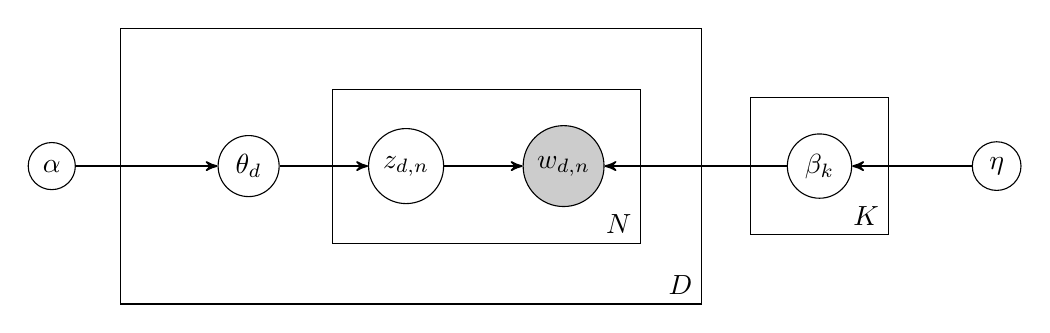
\begin{tikzpicture}
    [
      observed/.style={minimum size=15pt,circle,draw,fill=gray!40},
      latent/.style={minimum size=15pt,circle,draw},
      hyper/.style={minimum size=15pt,circle,draw},
      post/.style={->,>=stealth',semithick},
    ]

    \node (wdn) [observed] at (0.5,0) {$w_{d,n}$};
    \node (zdn) [latent] at (-1.5,0) {$z_{d,n}$};
    \node (theta) [latent] at (-3.5,0) {$\theta_d$};%zprior
    \node (alpha) [latent] at (-6,0) {$\alpha$}; %zhyper     \node (alpha) [label=left:$\alpha$] at (-6,0) {}; %zhyper
    \node (beta) [latent] at (3.75,0) {$\beta_k$}; %whyper
    \node (eta) [latent] at (6,0) {$\eta$}; {};
    
    \path
    (zdn) edge [post] (wdn)  
    (alpha) edge [post] (theta)
    (theta) edge [post] (zdn)
    (beta) edge [post] (wdn)
    (eta) edge [post] (beta)
    ;

    \node [draw,fit=(wdn) (theta), inner sep=35pt] (document-plate) {};
    \node [above left] at (document-plate.south east) {$D$};
    \node [draw,fit=(wdn) (zdn), inner sep=13pt] (word-plate) {};
    \node [above left] at (word-plate.south east) {$N$};
    \node [draw, fit=(beta), inner sep = 13pt] (topic-plate) {};
    \node [above left] at (topic-plate.south east) {$K$};

  \end{tikzpicture}
  \caption[LDA graphical model]{Graphical model of LDA. Shaded variables represent observed variables while non-shaded represent hidden or \textit{latent} variables. The rectangles, or "plates", represent replication for each generated variable. For example, the $D$ represents that each variable within are repeated $D$ times, for each document. $N$ represents words while $K$ represents topics.}
\label{dirichlet_notation}
\end{figure}

\subsubsection{Model Estimation}

In Bayesian statistics, conditional probability, or the \textit{posterior probability}, is given the general form of $P(A|B)$. As mentioned before, LDA is a Bayesian model, expanding upon Bayes' theorem. Using the previously mentioned variables, the posterior probability is calculated as shown in Equation \ref{posterior} (\cite{blei2012}). In this equation, the numerator represents the joint distribution of all random variables while the denominator represents the \textit{marginal probability} of observed terms. In other words, this denominator shows the probability of seeing any of the words within the corpus under any of the constructed \textit{K} topics. The expanded form of the joint distribution can be seen in Equation \ref{joint_distribution}. Since the only observed variable is $w_{d,n}$, this presents an obvious problem as the rest of the variables are unobserved so they must be calculated using $w_{d,n}$. Blei, Ng, et al. (2003) state that calculating the conditional probability as outlined in Equation \ref{posterior} is intractable and must instead be inferred using approximation algorithms. 

\begin{equation} \label{posterior}
p(\beta_{1:K}, \theta_{1:D}, z_{1:D} | w_{1:D}) = \frac{p(\beta_{1:K}, \theta_{1:D}, z_{1:D}, w_{1:D})}{p(w_{1:D})}
\end{equation}

\begin{equation} \label{joint_distribution}
p(\beta_{1:K}, \theta_{1:D}, z_{1:D}, w_{1:D})=\prod\limits_{k=1}^{K} p(\beta_k)\prod\limits_{d=1}^{D} p(\theta_d)\left(\prod\limits_{n=1}^{N}p(z_{d,n}|\theta_d)p(w_{d,n}|\beta_{1:K},z_{d,n})\right)
\end{equation}


One of these approximation algorithms that can be used to approach the issue of inferring this probability is a Markov chain Monte Carlo (MCMC), which aims "to simulate direct draws from some complex distribution of interest" (\cite{walsh2002}), with the distribution of interest being the Dirichlet distribution. A specific type of MCMC algorithm often used with LDA is the Gibbs sampling method. This algorithm helps obtain approximate observations from a multivariate probability distribution (such as the Dirichlet) to help approximate joint probabilities like in Equation \ref{posterior}. This method also can be applied to approximate the latent variables within the LDA model. For more information about MCMC and Gibbs sampling, see Walsh (2002). 

\subsection{Model Assessment}

To gauge the effectiveness of a constructed LDA model, there are multiple measures but one stands out to optimize the readability and interpretability of a topic. This aptly named measure is \textit{topic coherence}. Multiple different measures of topic coherence exist, however, this paper will focus on using Röder et al.'s (2015) measure for topic coherence, where they combine several other frequently used topic coherence methods to create topics that they have shown to have a higher correlation with human interpretability. This method is an intrinsic method of evaluating topic models (as opposed to extrinsic, which uses an external reference corpus) by using sliding windows to create \textit{virtual documents} based on the window size. For example, a sliding window size of 10 would move along the text and create vectors consisting of 10 words. Using an expansion of cosine similarity, these vectors are compared with one another and then aggregated and averaged into a singular $C_V$ score, where $C_V \in [0, 1]$. This $C_V$ score will be referred to as simply \textit{coherence score}. More information about the $C_V$ coherence measure can be found in Röder et al. (2015).

While data for LDA models is often used on large archives of documents, it can still be used on smaller sets of documents or documents with smaller lengths. One application of using LDA models on shorter text can be found in Sokolova et al. (2016) where the authors use LDA models on Twitter data. Since tweets can only have a maximum of 280 characters, the text is very short and yet the authors still utilize this data and use coherence scores as their method of assessing the constructed models. 

\subsubsection{Alternatives to Topic Coherence}

Besides coherence scores, the other measures which are commonly used to give a quantitative metric of assessing LDA models include computing hold out probability and model perplexity. The former is discussed in Wallach et al. (2009) \nocite{wallach2009} where the authors compute hold out probability based on a trained LDA model. This will calculate $P(W|W')$, where $W$ represents the test set documents and $W'$ represents training documents. Effective LDA models will show high probabilities for this metric, as it supports that the tokens from the training set documents can account for tokens introduced from the test set documents. Closely related to this metric is perplexity as applied by Blei, Ng, et al. (2003). The perplexity score for $W$ test set documents is calculated in Equation \ref{eq:perplexity} using the total number of tokens $N$ per document $d$ and is "equivalent to the inverse of the geometric mean per-word likelihood," (ibid.). When the trained model is applied to the test set, the perplexity score essentially shows how "perplexed" the model is by the introduction of tokens in these new documents. In this case, a lower perplexity is indicative of a better performing LDA model as it will able to fit the test set data better versus a higher perplexity score. Using this method on smaller data sets may be undesirable as it reduces the amount of textual data the LDA model can be trained from which can lead to a decrease in topic cohesion compared to using the entire data set for training.

\begin{equation} \label{eq:perplexity}
perplexity = \exp\left({\frac {\sum_{d=1}^W\log{p(W'_d)}}{\sum_{d=1}^W N_d}}\right)
\end{equation}

While these methods remained commonplace for evaluating LDA models, Chang et al. (2009) \nocite{Chang2009} argues that these methods have issues when associated with human interpretation. In experiments with human subjects, subjects were asked to identify an intrusive word into created topics. For example, the word set \texttt{\{cat, dog, buffalo, fox, lion, house}\} is presented to subjects and would then identify \textit{house} as the intruding word as it is the only non-animal word. With word sets that have no clear intruding word such as \texttt{\{money, gym, road, purple, Norway, light}\}, subjects would have trouble identifying the intruding word and often pick a word at random, indicating a topic with low topic coherence (ibid.). Using a similar measure as Wallach et al. (2009), Chang et al. use predictive log-likelihood and compare it against the results of the human experiments using word intrusion. They found that models with high log-likelihood were negatively correlated with human interpretability. Based on these findings as well as the findings from Röder et al. (2015), using topic coherence scores is the metric of interest for assessing the created LDA models. 

\section{Methodology and Empirical Results}

To create an LDA model, Python's gensim module can be used to create LDA models and assess the $C_V$ coherence score of the resulting models. However, it is not possible to use a string of long text and create an effective LDA model out of it. Pre-processing steps must be taken to create the LDA model, such as putting the textual data into a format that can be read by Python, cleaning the data, and placing the text into a corpus for the creation of the LDA model. All the data relating to this paper was provided by organizers of these events as well as online resources found on web pages related to these events.

\subsection{Pre-Processing} 

Each data set contained abstracts or extended abstracts from papers submitted to the conference organizers. To read in the data into Python, I first took the text from each accepted conference paper, keeping all relevant textual data from each respective data set and converted it into a \texttt{.txt} file.  The only portions of the data that were not included were headers/footers on the page. Originally, the data was either in a \texttt{.pdf} or \texttt{.xlsx} format. While \texttt{.pdf} files are not easily read into Python as \texttt{.xlsx} files, all files were converted into a \texttt{.txt} format for uniformity as I created functions that could be used across all three data sets with \texttt{.txt} files as the input. 

After loading in the data sets from their respective directories into Python, the data was contained in array format with each entry as one long string containing all the text from the original file. To make the data in a manageable form, the data must be tokenized such that the data is converted into a matrix where each row corresponds to the document itself and each column is an individual word with all columns in sequential order of how the text appears. It is important to note that the order of the text in an LDA model is not important as it is a bag-of-words (BoW) model where the model is constructed regardless of the order of the words. However, future pre-processing steps depend on the words being in sequential order.

\subsubsection{Cleaning and Tokenizing} 

Before tokenizing the data, it must be cleaned first. To clean the data, capitalization, punctuation (besides hyphens which were deleted to preserve the content of the compound word), and numbers were removed. This will make it so that words that have the same semantic meaning (such as \textit{model} and \textit{Model}) will be recognized as the same word (\textit{model}) by Python. Without this step, two or more instances of the same word could appear in a topic as separate words. Numbers were also removed as they would not be important to have within the topics given the data sets. 

With the data sets cleaned, they could then be tokenized to split each document by word into matrix format with each document in the rows and each word contained in the document in the columns as exemplified in Table \ref{tab:cleaned data}. Many of the words originally contained in this matrix were words that are commonly used in the English language daily such as prepositions. These commonly used words are known as \textit{stop words}. Stop word examples include \textit{it, or, and, the, her, on}, etc. To ensure that these words do not appear in the resulting LDA models, these stop words are removed from the data sets. A full list of stop words is given in Appendix \ref{stop_words}. These words are useless to include within the data set as they give no meaning to the topics and are therefore removed. Additionally, words were removed from the corpus if they were present in over two-thirds of all documents in that data set. This was done to prevent common words not included in the stop word list that would not add to topic cohesion due to prevalence. Words such as \textit{question} or \textit{research}  would likely be used across many papers but do not provide information on the underlying topic of the paper. 	

The last cleaning step is to create \textit{n}-grams for the data set. An \textit{n}-gram is a string of \textit{n} consecutive words. Common examples of \textit{n}-grams include bigrams and trigrams where $n=2$ and $n=3$, respectively. For this paper, I only focus on using bigrams in the data set and ensure the bigrams are only constructed if at least three instances of them appear in the entire data set. For example, if the words \textit{stochastic} and \textit{programming} appear consecutively in this order more than three times in a data set, gensim will construct a bigram of these two words connected with an underscore such that the bigram becomes \textit{stochastic\textunderscore programming}. Since this step is performed after the punctuation removal, these two words combined essentially become their own word to be recognized by the LDA model to help construct more unique topics. 

\begin{table}[H]
\centering
\resizebox{\textwidth}{!}{%
\begin{tabular}{@{}llllll@{}}
\toprule
Document & \multicolumn{1}{c}{Word 1} & \multicolumn{1}{c}{Word 2} & \multicolumn{1}{c}{Word 3} & \multicolumn{1}{c}{Word 4} & \multicolumn{1}{c}{Word 5} \\ \midrule
0 & workload\_balance & megacitie & adepartment & industrial & year \\
1 & model & passengers\_preference & smartphone & base & service \\
2 & solve & aim & create & set & route \\
3 & electric & carshare & charge & reposition & problem \\ \bottomrule
\end{tabular}%
}
\caption[Cleaned data matrix example]{Subset of matrix showing cleaned textual data after removal of stop words. Note that words connected by underscores are formed bigrams.}
\label{tab:cleaned data}
\end{table}

\subsubsection{Lemmatization and POS-Tagging}

In addition to cleaning the data, additional pre-processing steps can help with the construction of topics in the LDA model. One method is lemmatizing the words in the data set. Lemmatization will essentially reduce a word to its basic form, its \textit{lemma}. This process removes any past/present/future tense on verbs, possessive and plural forms on nouns, or any other inflected forms on words. For example, the words \textit{walking, walked, walks}, will all be reduced to their lemma, \textit{walk}. This process is done in Python using an external lemmatizer produced by spaCy (\cite{spacy}). 

A second step to pre-process the data is similar to a cleaning step as it will remove words from the data set if it does not fit a certain part-of-speech (POS). Parts-of-speech includes adverbs, adjectives, verbs, nouns, pronouns, proper nouns, etc.  Each word in the data set is tagged with a POS tag using the POS tagger developed by the Natural Language Toolkit (NLTK) (\cite{nltk}). The only POS tags that were allowed to remain in the data set were nouns, adjectives, verbs, and adverbs. Proper nouns were not included (except with LOGMS2017) as author names should not be included in the topics and the city names that appeared in the data set were primarily in reference to the author's home university, such as \textit{University of Shanghai}. One downside of removing proper nouns from the data set would remove all countries as well. If a certain country was mentioned many times it would be removed. Looking briefly through the data sets showed that ICSP2019 and TSL2018 did not have many papers focused on specific country studies, however, the LOGMS2017 data set did so proper nouns were kept for this data set. 

After pre-processing, the corpora are constructed from the individual data sets. The corpus from each conference becomes the main input for the corresponding LDA model as the words in each topic are constructed using these corpora. These words are the observed variable in the model, $w_{d,n}$. 

\subsection{LDA Models Using Optimized \textit{K}}

One common issue surrounding the creation of LDA models is what to set the number of $K$ topics to. In the scope of conference scheduling, the number of conference blocks and sessions is set in advance, and therefore $K$ can be decided based on the total number of planned conference sessions. This portion of the paper assumes that $K$ is not yet decided and different values of $K$ are tested in order to see which creates the highest scoring model in terms of coherence score. A later section will present results from LDA models where $K$ is equal to the total number of sessions within each conference. This is done to present any differences between the different methods to see if there is any difference in human interpretation between topics and how the value of $K$ affects document-topic placement.

Additionally, the Dirichlet priors $\alpha$ and $\eta$ must be decided in advance. As discussed previously, these parameters affect the shape of the Dirichlet distribution and, to build an optimal model, efficient values of $\alpha$ and $\eta$ must be chosen. To see how each parameter will affect the coherence score, multiple values of symmetric $\alpha$ and $\eta$ are chosen in conjunction with values of $K$ and a model is created to see the coherence of the resulting model. The combination of $K$, $\alpha$, and $\eta$ which results in the highest in-sample scoring LDA model on each data set is chosen and results from some of these topics and document placements are analyzed. Only a few topics from the LDA model for each data set are analyzed rather than all for brevity. 

Despite each data set not being large (see Table \ref{tab:doc_statistics}), constructing an LDA model and calculating its coherence score using many different parameters can be computationally expensive. Therefore, the symmetric $\alpha$ and $\eta$ values tested for maximizing coherence score are limited to be $\alpha = \eta = \{0.01, 0.25, 0.50, 0.75, 0.99\}$. Each of these values are tested alongside with different values of $K$ to show which combination of $K$, $\alpha$, and $\eta$ result in the highest coherence scoring LDA model. I chose to not have these values to not equal or exceed $1$ as a high $\alpha$ would cause words to begin to cluster around the center, making it difficult to distinguish the topics from one another and generally be unhelpful when displaying topic proportions per document, $\theta_{d,k}$. $\eta$ was limited to these values as a higher $\eta$ would result in less sparse topics where, again, it would be unhelpful when showing topic proportions for the documents and creating cohesive topics. 

\begin{table}[H]
\centering
\resizebox{\textwidth}{!}{%
\begin{tabular}{@{}cccc@{}}
\toprule
\multicolumn{1}{l}{} & \textbf{ICSP2019} & \multicolumn{1}{l}{\textbf{TSL2018}} & \multicolumn{1}{l}{\textbf{LOGMS2017}} \\ \midrule
No. Docs & 260 & 49 & 96 \\
Total File Size & 352 KB & 217 KB & 203 KB \\ \midrule
\begin{tabular}[c]{@{}c@{}}Total Tokens \\ (Pre-Cleaning)\end{tabular} & 52015 & 41887 & 31092 \\
\begin{tabular}[c]{@{}c@{}}Avg. Tokens \\ (Pre-Cleaning)\end{tabular} & 200 & 855 & 324 \\
\begin{tabular}[c]{@{}c@{}}Tokens Std. Deviation \\ (Pre-Cleaning)\end{tabular} & 110 & 334 & 144 \\ \midrule
\begin{tabular}[c]{@{}c@{}}Total Tokens \\ (Post-Cleaning)\end{tabular} & 21264 & 15401 & 15053 \\
\begin{tabular}[c]{@{}c@{}}Avg. Tokens \\ (Post-Cleaning)\end{tabular} & 82 & 314 & 157 \\
\begin{tabular}[c]{@{}c@{}}Tokens Std. Deviation \\ (Post-Cleaning)\end{tabular} & 46 & 117 & 68 \\ \bottomrule
\end{tabular}%
}
\caption{Descriptive statistics of different data sets used.}
\label{tab:doc_statistics}
\end{table}

The value of $K$ primarily depends on the size of the data set used, with more documents typically requiring a larger number of topics to characterize the data. These values of $K$ must be less than or equal to the documents in the data set. When $K = \text{(\# of documents)}$ the LDA model becomes a \textit{membership model}  and when $K < \text{(\# of documents)}$, the LDA is known as a \textit{mixed-membership model} (\cite{blei2003}). 

With the values of $K$, $\alpha$, and $\eta$ chosen to be tested for coherence, each value is used and the model is created with its corresponding coherence score calculated. This part is iterated through until every combination of the parameters are tested. For example, the first iteration would have $K = 2$ ($K = 1$ omitted as it would not provide meaningful results), $\alpha = 0.01$, $\eta = 0.01$ and the second iteration of this algorithm would be $K = 3, \alpha = 0.01$, $\eta = 0.01$ and so forth. In ICSP2019 and LOGMS2017, experimentation showed having a $K$ ranging from 2 - 20 had lower coherence scores than $K \ge 20$, and to reduce computation time, this range was set to begin at 20. Using these parameters yields a total of 25 iterations per $K$ value tested. Each iteration creates an LDA model which also calculates the in-sample coherence score which takes roughly 10-13 seconds per iteration (depending on the data set) using a computer with 16 GB of RAM and an Intel i7 processor @ 3.70GHz. The results from these iterations and the parameters associated with the highest scoring model for each data set are shown in Table \ref{tab:varied K parameter_table}. Line plots showing the highest performing model per every $k$ is shown in Appendix \ref{Figures}. 


\begin{table}[H]
\centering
\begin{tabular}{@{}lccccc@{}}
\toprule
          & K Range      & Alpha & Eta  & K  & Coherence Score \\ \midrule
ICSP2019  & {[}20,100{]} & 0.25  & 0.99 & 70 & 0.4549          \\
TSL2018   & {[}2,30{]}   & 0.50  & 0.01 & 22 & 0.3410          \\
LOGMS2017 & {[}20,60{]}  & 0.25  & 0.99 & 49 & 0.3817          \\ \bottomrule
\end{tabular}
\caption[Parameters from LDA models]{Parameters used to obtain highest scoring LDA model and corresponding coherence score.}
\label{tab:varied K parameter_table}
\end{table}

The coherence scores were calculated using a sliding window of 50 tokens. Röder et al. (2015) construct their $C_V$ coherence score measure using a sliding window of 110. The authors note that different values for this sliding window can be used, but remark that a sliding window of at least 50 tokens should be used. Table \ref{tab:doc_statistics} shows that the average document from ICSP2019 does not have 110 tokens after cleaning and the sliding window is set to 50. This also accounts for smaller texts found in LOGMS2017 as texts one standard deviation below the mean have less than 110 tokens after cleaning. The histogram displaying the token counts per document after cleaning is shown in Appendix \ref{Figures}.

With the highest-scoring models identified, the parameters from Table \ref{tab:varied K parameter_table} are used for each of the respective corpora and the LDA model is created. From the LDA model, the latent variables can be inferred. This includes the topics $\beta_{1:K}$ and the topic assignments $\theta_{d,k}$ for each document. The topics are reported as a list with the most frequent words appearing at the top of the list for each topic. The top 10 words are reported on this list. In future sections, only the top five words are presented to preserve the readability of tables, especially with data sets that resulted in a high number of topics. A full list of the words and their corresponding topic-word probabilities are attached as a separate appendix. Examining the topics is an important step to give a human interpretation of the topic themselves as the resulting topics from the LDA model are useless unless conference organizers can make sense out of the topics. 

After the topics are presented and coherence scores are calculated, the next step is to organize each of the documents into different topics. In this case, each topic would be representative of a session for the conference. With topics where a large number of documents are assigned, multiple conference sessions can be dedicated to these topics. This is the case in the actual conference plan for ICSP2019 and LOGMS2017 where multiple sessions were dedicated to the same topic. These sessions do not run in parallel in case an attendee wanted to attend all talks on this topic. Document assignments to sessions are determined by the $\theta_{d,k}$ values for all documents $D$ over $K$ topics. The documents are assigned to the topic where the $\theta_{d,k}$ value is highest. For example, if document 1 has $\theta_{1,1} = 0.75$ for topic 1 and $\theta_{1,2} = 0.25$ for topic 2, document 1 would be placed into topic 1 and a session is created with all other documents placed into topic 1. An example of how the $\theta_{d,k}$ matrix is constructed is shown in Table \ref{tab:TSL2018 theta matrix} for TSL2018. The full matrix is included as an attached appendix for all data sets. All the topic probabilities per document (rows) sum to exactly 1 for all documents. While the entries may show a zero probability, this number is just very small to the point the LDA model in Python equates it to zero. Theoretically, it is impossible for a $\theta_{d,k}$ value to be zero (\cite{blei2003}). 

With documents assigned to topics, the titles for each document are presented in tabular form along with the $\theta_{d,k}$ values and the session titles these documents were assigned to. As the value for $K$ varies greatly between these data sets, only a handful of the total number of topics were analyzed from each conference for brevity.


\begin{table}[h]
\centering
\resizebox{\textwidth}{!}{%
\begin{tabular}{@{}lllllllllll@{}}
\toprule
 & \textbf{Topic 0} & \textbf{Topic 1} & \textbf{Topic 2} & \textbf{Topic 3} & \textbf{Topic 4} & \textbf{Topic 5} & \textbf{Topic 6} & \textbf{Topic 7} & \textbf{Topic 8} & \textbf{Topic 9} \\ \midrule
\textbf{Document 0} & 0 & 0 & 0 & 0 & 0 & 0 & 0 & 0 & 0 & 0 \\
\textbf{Document 1} & 0 & 0 & 0 & 0 & 0 & 0 & 0 & 0 & 0 & 0 \\
\textbf{Document 2} & 0 & 0 & 0.0365 & 0 & 0 & 0 & 0.0104 & 0 & 0 & 0 \\
\textbf{Document 3} & 0.0350 & 0.0832 & 0.2328 & 0 & 0.0249 & 0 & 0 & 0 & 0.1031 & 0 \\
\textbf{Document 4} & 0 & 0 & 0 & 0 & 0 & 0 & 0 & 0 & 0 & 0 \\
\textbf{Document 5} & 0 & 0 & 0 & 0 & 0 & 0 & 0 & 0 & 0 & 0.8914 \\
\textbf{Document 6} & 0.0189 & 0 & 0.0634 & 0 & 0 & 0 & 0 & 0 & 0 & 0.0430 \\
\textbf{Document 7} & 0 & 0.0661 & 0 & 0 & 0 & 0 & 0 & 0 & 0.6875 & 0.0461 \\
\textbf{Document 8} & 0 & 0 & 0.0568 & 0 & 0 & 0 & 0 & 0 & 0.2572 & 0 \\
\textbf{Document 9} & 0 & 0 & 0 & 0 & 0.0103 & 0 & 0.0796 & 0 & 0 & 0 \\ \bottomrule
\end{tabular}%
}
\caption[Document-topic probabilities matrix example]{Subset of document-topic probabilities $\theta_{d,k}$ for TSL2018.}
\label{tab:TSL2018 theta matrix}
\end{table}



\subsubsection{ICSP2019}

Using the papers from the ICSP2019 conference, the model with the highest coherence score was associated with $K = 70$ for the number of topics and using the Dirichlet parameters $\alpha = 0.25$ and $\eta = 0.99$. With these parameters, the resulting coherence score is 0.4549. The topics from the resulting LDA model, including the top five words contained within these topics and the topic-word probabilities, can be seen in \ref{tab:ICSP varied K topics}. All the topics which were repeated in the LDA model were removed except for one instance which is shown highlighted in the table. 

\begin{table}[H]
\centering
\resizebox{\textwidth}{!}{%
\begin{tabular}{@{}llllll@{}}
\toprule
\textbf{} & \multicolumn{1}{c}{\textbf{Word 1}} & \multicolumn{1}{c}{\textbf{Word 2}} & \multicolumn{1}{c}{\textbf{Word 3}} & \multicolumn{1}{c}{\textbf{Word 4}} & \multicolumn{1}{c}{\textbf{Word 5}} \\ \midrule
\rowcolor[HTML]{FCFF2F} 
\textbf{Topic 0} & 0.001*"convexconcave" & 0.001*"correlate" & 0.001*"advance" & 0.001*"plane" & 0.001*"ecrm" \\
\textbf{Topic 4} & 0.017*"optimisation" & 0.010*"multistage" & 0.008*"bound" & 0.006*"class" & 0.004*"point" \\
\textbf{Topic 9} & 0.004*"item" & 0.002*"user" & 0.002*"offer" & 0.002*"online" & 0.002*"mechanism" \\
\textbf{Topic 34} & 0.006*"game" & 0.003*"player" & 0.003*"tree" & 0.002*"forward" & 0.002*"agent" \\
\textbf{Topic 35} & 0.016*"model" & 0.016*"system" & 0.010*"market" & 0.008*"uncertainty" & 0.008*"scenario" \\
\textbf{Topic 39} & 0.002*"investor" & 0.002*"housing" & 0.002*"reverse" & 0.001*"lifetime" & 0.001*"purchase" \\
\textbf{Topic 41} & 0.003*"reposition" & 0.002*"unit" & 0.002*"inventory" & 0.001*"region" & 0.001*"ondemand" \\
\textbf{Topic 49} & 0.014*"method" & 0.014*"model" & 0.011*"solve" & 0.010*"approach" & 0.010*"solution" \\
\textbf{Topic 54} & 0.008*"statistical" & 0.007*"discuss" & 0.006*"learning" & 0.005*"talk" & 0.005*"smooth" \\
\textbf{Topic 58} & 0.007*"pde" & 0.004*"gas" & 0.003*"carlo" & 0.002*"load" & 0.002*"hierarchy" \\
\textbf{Topic 69} & 0.002*"budget" & 0.001*"uncertainty\_set" & 0.001*"adjustable" & 0.001*"confirm" & 0.001*"match" \\ \bottomrule
\end{tabular}%
}
\caption[ICSP2019 varied K topics]{First 5 words from ICSP2019 LDA model topics using $K = 70$, $\alpha = 0.25$, and $\eta = 0.99$. Duplicate topics are removed. Note that the highlighted topic is the topic which is repeated for all missing topic numbers.}
\label{tab:ICSP varied K topics}
\end{table}

Out of the 70 topics created by this model, only 11 of these were unique as they were not identical to topic 0. The topics presented are a mix of specific topics and also \textit{catch-all} topics. A catch-all topic is a topic constructed of very general and common words that have little to no specific relationship to each other. The presence of some catch-alls can be seen in the presented topics, especially in the scope of stochastic programming: the theme of the ICSP conference. Topic 49 is a catch-all topic, with the words being very general to stochastic programming and little specific relationship to each other. Other topics including topics 34 or 39 contain words, which when placed together, are shown to be related to a specific topic. In topic 34, the words \textit{game, player, tree,} and \textit{agent} could be indicative of a topic descriptive of game theory. Topic 39 shows words such as \textit{investor, housing, reverse, lifetime, purchase,} and \textit{equity} (not shown in table) which is indicative of housing purchases, mortgages, or real estate. With the LDA model created, the $\theta_{d,k}$ values showing the probability for each document being contained within topic $k$ are calculated. From these probabilities, documents are placed into topics where the probability is highest. The document assignments into topics can be shown in Figure \ref{fig:ICSP2019 varied K placements}.

\begin{figure}[H]

  \centering
  \includegraphics[width=0.65\linewidth]{ICSP_placement.png}
\caption[ICSP2019 varied K document-topic distribution]{Document-topic distribution based on highest $\theta_{d,k}$ value for each document for ICSP2019 where $K = 70$.}
\label{fig:ICSP2019 varied K placements}
\end{figure}

A large majority of the documents were placed into topic 49, a catch-all topic especially in the scope of stochastic programming. All of the top five words within this topic are too general to discern a specific topic from, as these are words that would be found in likely any scientific research paper. The same is the case for topics 35, however topic 54 may be descriptive of machine learning algorithms as it includes words such as \textit{statistical, learning, smooth, estimation}, and \textit{algorithm}. Meanwhile, the rest of the topics with documents assigned to them are very small. Topics 9 and 4 have two documents assigned to them while topics 58, 39, and 34 only have one. For the ICSP2019 conference, most of the sessions contained 3-4 talks, with few containing two speakers. Note that topic 0 or any of the identical topics appeared in the document-topic distribution. Looking at the topic-word probabilities in topic 0, all words have a probability of 0.001 which is much lower than some of these other topics which contain words that have a probability of 0.014 or higher which can heavily influence document-topic placement.

Deep diving into topics 54, 9, and 4, the document titles and the ICSP2019 actual document groupings are presented in Tables \ref{tab:ICSP2019 topic 54 titles varied K}, \ref{tab:ICSP2019 topic 9 titles varied K}, and \ref{tab:ICSP2019 topic 4 titles varied K}. Topics 49 and 35 are ignored as the number of documents assigned to these topics (176 and 60, respectively) would be too large to assign multiple sessions to, especially with such a general topic. Using 4 talks per session, this would result in 44 sessions allocated to this topic for topic 49 and 15 sessions allocated to topic 35. Topics 58, 39, and 34 are ignored as sessions should contain more than one speaker. 

\begin{table}[H]
\centering
\resizebox{\textwidth}{!}{%
\begin{tabular}{|c|c|c|c|}
\hline
\textbf{d} & \textbf{$\theta_{d,54}$} & \textbf{Document Title} & \textbf{ICSP2019 Session Title} \\ \hline
\textbf{\begin{tabular}[c]{@{}c@{}}Document\\  221\end{tabular}} & 0.7395 & \begin{tabular}[c]{@{}c@{}}Advances In Understanding Structural \\ Properties Of Probability Functions\end{tabular} & Nonlinear Programming With Probability Functions \\ \hline
\textbf{\begin{tabular}[c]{@{}c@{}}Document \\ 145\end{tabular}} & 0.5857 & \begin{tabular}[c]{@{}c@{}}Wasserstein Distributionally Robust Optimization: \\ Theory And Applications   In Machine Learning\end{tabular} & Data-Driven Distributionally Robust Optimization \\ \hline
\textbf{\begin{tabular}[c]{@{}c@{}}Document \\ 163\end{tabular}} & 0.5765 & \begin{tabular}[c]{@{}c@{}}The Effect Of Curvature On The Convergence\\  Rate Of Stochastic Gradient   Descent\end{tabular} & Statistics And Machine Learning \\ \hline
\textbf{\begin{tabular}[c]{@{}c@{}}Document \\ 250\end{tabular}} & 0.5603 & Topics In Stochastic Gradient Approximation & \begin{tabular}[c]{@{}c@{}}Stochastic Approximation Schemes For \\ Stochastic Optimization,   Variational,\\  And Game-Theoretic Problems\end{tabular} \\ \hline
\textbf{\begin{tabular}[c]{@{}c@{}}Document \\ 209\end{tabular}} & 0.5546 & (Deep) Learning With More Parameters Than Data & \begin{tabular}[c]{@{}c@{}}Interfaces Between Learning And\\  Stochastic Optimization\end{tabular} \\ \hline
\textbf{\begin{tabular}[c]{@{}c@{}}Document \\ 168\end{tabular}} & 0.5504 & \begin{tabular}[c]{@{}c@{}}Zeroth-Order Recursive Optimization Of \\ Mean-Semideviation Risk Measures\end{tabular} & \begin{tabular}[c]{@{}c@{}}Stochastic Approximation Schemes For \\ Stochastic Optimization,   Variational, \\ And Game-Theoretic Problems\end{tabular} \\ \hline
\textbf{\begin{tabular}[c]{@{}c@{}}Document \\ 216\end{tabular}} & 0.5316 & \begin{tabular}[c]{@{}c@{}}Consistency of Stationary Solutions of Coupled\\  Nonconvex Nonsmooth   Empirical Risk Minimization\end{tabular} & \textit{Plenary Session} \\ \hline
\textbf{\begin{tabular}[c]{@{}c@{}}Document \\ 244\end{tabular}} & 0.4897 & \begin{tabular}[c]{@{}c@{}}Multi-Composite Nonconvex Optimization \\ For Training Deep Neural Network\end{tabular} & Statistics And Machine Learning \\ \hline
\textbf{\begin{tabular}[c]{@{}c@{}}Document \\ 78\end{tabular}} & 0.4782 & \begin{tabular}[c]{@{}c@{}}Distributionally Robust Inverse Covariance Estimation: \\ The Wasserstein   Shrinkage Estimator\end{tabular} & Applications Of Distributionally Robust Optimization \\ \hline
\textbf{\begin{tabular}[c]{@{}c@{}}Document \\ 143\end{tabular}} & 0.4555 & Learning Enabled Optimization & Predictive Stochastic Programming \\ \hline
\textbf{\begin{tabular}[c]{@{}c@{}}Document \\ 31\end{tabular}} & 0.4201 & \begin{tabular}[c]{@{}c@{}}Zeroth-Order Nonconvex Stochastic Optimization:\\  Handling Constraints, High-Dimensionality, \\ And Saddle-Points\end{tabular} & \begin{tabular}[c]{@{}c@{}}Bounds And Approximations In Optimization\\  Under Uncertainty\end{tabular} \\ \hline
\textbf{\begin{tabular}[c]{@{}c@{}}Document \\ 98\end{tabular}} & 0.4045 & \begin{tabular}[c]{@{}c@{}}Optimistic Likelihood Problems Using \\ (Geodesiclly) Convex Optimization\end{tabular} & Methodological Advances In Robust Optimization \\ \hline
\textbf{\begin{tabular}[c]{@{}c@{}}Document\\  205\end{tabular}} & 0.3716 & \begin{tabular}[c]{@{}c@{}}The role of decomposition methods in\\  stochastic programming\end{tabular} & \textit{Plenary Session} \\ \hline
\textbf{\begin{tabular}[c]{@{}c@{}}Document \\ 9\end{tabular}} & 0.3643 & \begin{tabular}[c]{@{}c@{}}Kernel Estimation In Stochastic Optimization\\  With Composite Risk   Functionals\end{tabular} & Advances In Risk-Averse Optimization \\ \hline
\textbf{\begin{tabular}[c]{@{}c@{}}Document \\ 109\end{tabular}} & 0.3471 & \begin{tabular}[c]{@{}c@{}}Fractional Kelly Investing And \\ Wealth Benchmarking\end{tabular} & \begin{tabular}[c]{@{}c@{}}New Frontiers In Financial Decision Making \\ Under Uncertainty: Ambiguity, Stochastic Dominance \\ And Complex Nonlinear Portfolio Management\end{tabular} \\ \hline
\textbf{\begin{tabular}[c]{@{}c@{}}Document \\ 183\end{tabular}} & 0.3441 & Software for Stochastic Programming & \textit{Pre-Conference Tutorial} \\ \hline
\textbf{\begin{tabular}[c]{@{}c@{}}Document \\ 167\end{tabular}} & 0.3294 & \begin{tabular}[c]{@{}c@{}}Advances In Wasserstein Distributionally \\ Robust Optimization\end{tabular} & Data-Driven Distributionally Robust Optimization \\ \hline
\end{tabular}%
}
\caption[ICSP2019 topic 54 distribution with varied K]{Titles and $\theta_{d,54}$ values for documents assigned to topic 54, with the actual ICSP2019 session assignments.}
\label{tab:ICSP2019 topic 54 titles varied K}
\end{table}

\begin{table}[H]
\centering
\resizebox{\textwidth}{!}{%
\begin{tabular}{|c|c|c|c|}
\hline
\textbf{d} & \textbf{$\theta_{d,9}$} & \textbf{Document Title} & \textbf{ICSP2019 Session Title} \\ \hline
\textbf{Document 105} & 0.7636 & \begin{tabular}[c]{@{}c@{}}A Two-Layer Multi-Armed Bandit Approach \\ For Online Multi-Item Pricing\end{tabular} & \begin{tabular}[c]{@{}c@{}}New Applications Of Distributionally\\  Robust Optimization\end{tabular} \\ \hline
\textbf{Document 196} & 0.4532 & \begin{tabular}[c]{@{}c@{}}Robust Active Preference Elicitation To Learn\\  The Moral Priorities Of   Policy-Makers\end{tabular} & Doing Good With Good Ro \\ \hline
\end{tabular}%
}
\caption[ICSP2019 topic 9 distribution with varied K]{Titles and $\theta_{d,9}$ values for documents assigned to topic 9, with the actual ICSP2019 session assignments.}
\label{tab:ICSP2019 topic 9 titles varied K}
\end{table}

\begin{table}[H]
\centering
\resizebox{\textwidth}{!}{%
\begin{tabular}{|c|c|c|c|}
\hline
\textbf{d} & \textbf{$\theta_{d,4}$} & \textbf{Document Title} & \textbf{ICSP2019 Session Title} \\ \hline
\textbf{Document 254} & 0.6262 & \begin{tabular}[c]{@{}c@{}}Multistage Saddle Point Problems And\\  Non-Rectangular Uncertainty Sets\end{tabular} & \begin{tabular}[c]{@{}c@{}}Stochastic Dynamic Programming Equations: \\ Decomposition Methods And   Applications\end{tabular} \\ \hline
\textbf{Document 89} & 0.5472 & \begin{tabular}[c]{@{}c@{}}A Primal-Dual Lifting Scheme For\\  Two-Stage Robust Optimization\end{tabular} & \begin{tabular}[c]{@{}c@{}}Applications Of Distributionally\\  Robust Optimization\end{tabular} \\ \hline
\end{tabular}%
}
\caption[ICSP2019 topic 4 distribution with varied K]{Titles and $\theta_{d,4}$ values for documents assigned to topic 4, with the actual ICSP2019 session assignments.}
\label{tab:ICSP2019 topic 4 titles varied K}
\end{table}

While according to the words included in topic 54 seemed to be descriptive of machine learning, looking at the titles and actual conference session assignments in Table \ref{tab:ICSP2019 topic 54 titles varied K} provides some evidence supporting this but also evidence against this as well.  Some of the documents in this table show that they were grouped up together as the actual ICSP2019 conference organized these documents. For example, documents 163 and 244 are assigned to be under the session \textit{Statistics and Machine Learning} which is also likely why \textit{learning} or \textit{statistical} appeared in this topic, supporting that this topic could be related to machine learning. Other groupings also appear from the ICSP2019 conference schedule, however, these are unrelated to statistics and machine learning. \textit{Stochastic Approximation Schemes For Stochastic Optimization, Variational, And Game-Theoretic Problems} and \textit{Data-Driven Distributionally Robust Optimization} are the only other groupings from the original ICSP2019 conference schedule. From the original ICSP2019 sessions these documents were assigned to, 9 out of 16 of the original session titles grouped up by topic 54 include \textit{optimization} in the title which supports that the LDA model was able to organize these documents in a somewhat cohesive manner. However, given the nature of this conference, the frequency at which \textit{optimize} appears in topics and session titles is unsurprising given over 150 documents out of the full 260 contain \textit{optimize} or \textit{optimise} at least once meaning these groupings could have occurred due to similar words found in almost all papers.

With topics 9 and 4 in Tables \ref{tab:ICSP2019 topic 9 titles varied K} and \ref{tab:ICSP2019 topic 4 titles varied K}, respectively, the documents grouped together seem to have little to no relevance with each other. Additionally, these documents were placed into different sessions according to the actual ICSP2019 conference schedule. With the small variation between assigned topics and the low amount of total topics documents were assigned to, it becomes difficult to create a meaningful and engaging conference for attendees where sessions are grouped by content similarity.

\subsubsection{TSL2018}

The model resulting in the highest coherence score for the TSL2018 data set were with $K = 22$, $\alpha = 0.50$, and $\eta = 0.01$. These parameters result in a coherence score of 0.3410, lower than the ICSP2019 data set. The topics and the top five words contained within these topics can be seen in Table \ref{tab:TSL varied K topics} along with the topic-word probabilities of these words. 

\begin{table}[H]
\centering
\resizebox{\textwidth}{!}{%
\begin{tabular}{@{}llllll@{}}
\toprule
\multicolumn{1}{c}{} & \multicolumn{1}{c}{\textbf{Word 1}} & \multicolumn{1}{c}{\textbf{Word 2}} & \multicolumn{1}{c}{\textbf{Word 3}} & \multicolumn{1}{c}{\textbf{Word 4}} & \multicolumn{1}{c}{\textbf{Word 5}} \\ \midrule
\textbf{Topic 0} & 0.026*"vehicle" & 0.023*"demand" & 0.017*"system" & 0.014*"distribution" & 0.013*"locker" \\
\textbf{Topic 1} & 0.054*"passenger" & 0.052*"service" & 0.027*"transportation" & 0.021*"price" & 0.021*"discount" \\
\textbf{Topic 2} & 0.082*"vehicle" & 0.033*"congestion" & 0.029*"charge" & 0.027*"zone" & 0.026*"emission" \\
\textbf{Topic 3} & 0.020*"sequence" & 0.018*"set" & 0.018*"route" & 0.016*"approach" & 0.015*"road" \\
\textbf{Topic 4} & 0.099*"facility" & 0.050*"client" & 0.044*"demand" & 0.033*"formulation" & 0.021*"capacity" \\
\textbf{Topic 5} & 0.054*"delivery" & 0.042*"demand" & 0.036*"customer" & 0.034*"courier" & 0.030*"price" \\
\textbf{Topic 6} & 0.043*"bundle" & 0.030*"design" & 0.028*"task" & 0.020*"scenario" & 0.018*"service" \\
\textbf{Topic 7} & 0.001*"solution" & 0.001*"system" & 0.001*"delivery" & 0.001*"instance" & 0.001*"solve" \\
\textbf{Topic 8} & 0.030*"delivery" & 0.026*"customer" & 0.019*"vehicle" & 0.013*"scenario" & 0.011*"city" \\
\textbf{Topic 9} & 0.035*"deadline" & 0.020*"scenario" & 0.019*"risk" & 0.019*"space" & 0.018*"vrp" \\
\textbf{Topic 10} & 0.028*"reduce" & 0.025*"consolidation" & 0.023*"transportation" & 0.022*"truck" & 0.021*"carrier" \\
\textbf{Topic 11} & 0.031*"approach" & 0.026*"transportation" & 0.026*"profit" & 0.025*"ucc" & 0.022*"passenger" \\
\textbf{Topic 12} & 0.001*"carrier" & 0.001*"system" & 0.001*"transportation" & 0.001*"customer" & 0.001*"delivery" \\
\textbf{Topic 13} & 0.057*"order" & 0.037*"delivery" & 0.026*"system" & 0.025*"item" & 0.024*"route" \\
\textbf{Topic 14} & 0.023*"propose" & 0.017*"demand" & 0.017*"carrier" & 0.013*"customer" & 0.013*"approach" \\
\textbf{Topic 15} & 0.001*"vehicle" & 0.001*"demand" & 0.001*"facility" & 0.001*"type" & 0.001*"service" \\
\textbf{Topic 16} & 0.080*"solution" & 0.036*"transportation" & 0.032*"robustness" & 0.028*"constraint" & 0.027*"instance" \\
\textbf{Topic 17} & 0.106*"vehicle" & 0.095*"solve" & 0.090*"constraint" & 0.051*"visit" & 0.049*"capacity" \\
\textbf{Topic 18} & 0.042*"delivery" & 0.026*"request" & 0.025*"order" & 0.019*"approach" & 0.017*"customer" \\
\textbf{Topic 19} & 0.047*"customer" & 0.039*"share" & 0.034*"delivery" & 0.032*"ecommerce" & 0.031*"online" \\
\textbf{Topic 20} & 0.062*"system" & 0.029*"design" & 0.029*"logistic" & 0.029*"station" & 0.015*"optimization" \\
\textbf{Topic 21} & 0.034*"company" & 0.029*"function" & 0.028*"experience" & 0.025*"learn" & 0.020*"service" \\ \bottomrule
\end{tabular}%
}
\caption[ICSP2019 varied K topics]{First 5 words from TSL2018 LDA model topics using $K = 22$, $\alpha = 0.50$, and $\eta = 0.01$.}
\label{tab:TSL varied K topics}
\end{table}

Here, a similar issue with the ICSP2019 data set appears with some words contained within topics having specific topics while others are catch-all topics. However, there seems to be more specific topics than catch-all topics in this data set. Topic 17 is indicative of a topic relating to vehicle routing problems, as words in the topic include \textit{vehicle, solve, constraint, capacity, route,} (not pictured) and \textit{vehicle\textunderscore route} (not pictured). Another example of a specific topic would be in topic 19 which may be related to online shopping or e-Commerce with words such as \textit{customer, delivery, ecommerce, online,} and \textit{service} (not pictured). More examples include topic 2 being related to electric vehicles or topic 10 with consolidating goods in transportation for a supply chain. All of the included topics seem to be descriptive of some sort of logistical process or related to supply chain management. While initially this does seem like a success, this is due to the INFORMS TSL conference being focused on transportation sciences and logistics which accounts for the high number of transportation and logistics words in the topics. Therefore, some of these topics such as topic 7, 15, or 18 may be a catch-all topic as it shows general words relating to logistics and transportation sciences. After documents are allocated into topics based upon their highest $\theta_{d,k}$ value, the distribution over topics for documents is shown in Figure \ref{fig:TSL2018 varied K placements}.




\begin{figure}[H]

  \centering
  \includegraphics[width=0.65\linewidth]{TSL_placement.png}
\caption[TSL2018 varied K document-topic distribution]{Document-topic distribution based on highest $\theta_{d,k}$ value for each document for TSL2018 when $K=22$.}
\label{fig:TSL2018 varied K placements}
\end{figure}

The TSL2018 LDA model created a much more diverse number of topics compared to the ICSP2019 model without concentrating an majority of documents into one topic. Out of all the topics in the LDA model, 17 out of the total of 22 topics have at least one document assigned to them. While most topics are placed into topic 8, this shows that many documents are descriptive of the words contained in this topic which may facilitate the need for assigning multiple sessions to this topic. The same case may apply to the other topics with a high number of documents such as topic 14 or 0. Examining the top three topics in terms of documents assigned yields the results in Tables \ref{tab:TSL2018 topic 8 titles varied K} - \ref{tab:TSL2018 topic 0 titles varied K}. The other topics are omitted for brevity and topics with one document assigned to them are ignored.

% Please add the following required packages to your document preamble:
% \usepackage{graphicx}
\begin{table}[H]
\centering
\resizebox{\textwidth}{!}{%
\begin{tabular}{|c|c|c|c|}
\hline
\textbf{d} & \textbf{$\theta_{d,8}$} & \textbf{Document Title} & \textbf{TSL2018 Session Title} \\ \hline
\textbf{Document 12} & 0.9520 & \begin{tabular}[c]{@{}c@{}}Dynamic Pricing for Same-Day\\  Delivery Routing\end{tabular} & \begin{tabular}[c]{@{}c@{}}Business Modules of \\ Urban Logistics\end{tabular} \\ \hline
\textbf{Document 21} & 0.9321 & \begin{tabular}[c]{@{}c@{}}Same-Day Delivery with a Heterogeneous Fleet\\  of Drones and Vehicles\end{tabular} & Last Mile Delivery \\ \hline
\textbf{Document 37} & 0.9260 & \begin{tabular}[c]{@{}c@{}}Smart Locker Bank Design Optimization for \\ Urban Omnichannel Logistics\end{tabular} & \begin{tabular}[c]{@{}c@{}}Lockers \& \\ Mobile Facilities\end{tabular} \\ \hline
\textbf{Document 40} & 0.8682 & \begin{tabular}[c]{@{}c@{}}Opportunities and threats of mixing delivery \\ options in the e-commerce   era\end{tabular} & E-Commerce \\ \hline
\textbf{Document 7} & 0.6875 & \begin{tabular}[c]{@{}c@{}}Are delivery-drones a solution for the\\  last-mile problem in urban areas?\end{tabular} & Last Mile Delivery \\ \hline
\textbf{Document 25} & 0.5880 & \begin{tabular}[c]{@{}c@{}}Anticipating Emission-Sensitive Traffic Management \\ Strategies for Dynamic   Delivery Routing\end{tabular} & Green Urban Logistics \\ \hline
\textbf{Document 29} & 0.4815 & \begin{tabular}[c]{@{}c@{}}Omnichannel B2C Distribution: Modeling Approach \\ and Deployment Scenarios\end{tabular} & City Logistics \\ \hline
\textbf{Document 48} & 0.4791 & \begin{tabular}[c]{@{}c@{}}Multi-Commodity Two-Echelon Vehicle Routing \\ Problem with Time Windows\end{tabular} & \begin{tabular}[c]{@{}c@{}}Routing with Electric Vehicles \\ \& Time Windows\end{tabular} \\ \hline
\textbf{Document 39} & 0.4319 & \begin{tabular}[c]{@{}c@{}}Hyperconnected Last-Mile Delivery of \\ Large Items in Urban Area\end{tabular} & Urban Transportation \& Congestion \\ \hline
\textbf{Document 34} & 0.3418 & \begin{tabular}[c]{@{}c@{}}Scheduled Service Network Design with Resource\\  Management for Multimodal  City Logistics with \\ Inbound and Outbound Flows\end{tabular} & City Logistics \\ \hline
\end{tabular}%
}
\caption[TSL2018 topic 8 distribution with varied K]{Titles and $\theta_{d,8}$ values for documents assigned to topic 8, with the actual TSL2018 session assignments.}
\label{tab:TSL2018 topic 8 titles varied K}
\end{table}

\begin{table}[H]
\centering
\resizebox{\textwidth}{!}{%
\begin{tabular}{|c|c|c|c|}
\hline
\textbf{d} & \textbf{$\theta_{d,14}$} & \textbf{Document Title} & \textbf{TSL2018 Session Title} \\ \hline
\textbf{Document 26} & 0.9373 & \begin{tabular}[c]{@{}c@{}}On the economic and environmental benefits\\  of collaborative transportation and \\ the coalition configuration problem\end{tabular} & \begin{tabular}[c]{@{}c@{}}Collaborative Logistics \&\\  Ridesharing\end{tabular} \\ \hline
\textbf{Document 11} & 0.9247 & \begin{tabular}[c]{@{}c@{}}An Iterative Auction for Carrier Collaboration\\  in Truckload Pickup and   Delivery\end{tabular} & \begin{tabular}[c]{@{}c@{}}Collaborative Logistics \& \\ Ridesharing\end{tabular} \\ \hline
\textbf{Document 36} & 0.8801 & \begin{tabular}[c]{@{}c@{}}Sustainable Urban distribution under \\ demand and traveling time variations\end{tabular} & \textit{Not included in final TSL2018 conference} \\ \hline
\textbf{Document 33} & 0.6839 & \begin{tabular}[c]{@{}c@{}}Load Dependent Electric Vehicle Routing Problem \\ With Time Windows   Considering \\ Nonlinear Charging Function\end{tabular} & \begin{tabular}[c]{@{}c@{}}Routing with Electric Vehicles\\  \& Time Windows\end{tabular} \\ \hline
\textbf{Document 20} & 0.4726 & \begin{tabular}[c]{@{}c@{}}Selecting Shipments at An Urban Consolidation Center \\ for Last-mile   Delivery with Cost Uncertainty\end{tabular} & Consolidation for Urban Delivery \\ \hline
\textbf{Document 2} & 0.4395 & \begin{tabular}[c]{@{}c@{}}Solving the Consistent Vehicle Routing\\  Problem via Column Generation\end{tabular} & Methods for Vehicle Routing Problems \\ \hline
\end{tabular}%
}
\caption[TSL2018 topic 14 distribution with varied K]{Titles and $\theta_{d,14}$ values for documents assigned to topic 14, with the actual TSL2018 session assignments.}
\label{tab:TSL2018 topic 14 titles varied K}
\end{table}

\begin{table}[H]
\centering
\resizebox{\textwidth}{!}{%
\begin{tabular}{|c|c|c|c|}
\hline
\textbf{d} & \textbf{$\theta_{d,0}$} & \textbf{Document Title} & \textbf{TSL2018 Session Title} \\ \hline
\textbf{Document 46} & 0.9612 & Solving last-mile distribution problems after major earthquakes & Disruption Management \\ \hline
\textbf{Document 28} & 0.8991 & Federated locker system in last mile problem with Big Data & Lockers \& Mobile Facilities \\ \hline
\textbf{Document 13} & 0.8626 & Managing disruptions in urban road networks for real contexts & Disruption Management \\ \hline
\textbf{Document 42} & 0.7158 & \begin{tabular}[c]{@{}c@{}}A new inventory routing approach for managing multimodal\\  transportation   networks: Balancing dynamic inventory supply of \\ shared/transit vehicles for serving urban passenger demand\end{tabular} & \textit{Not included in final TSL2018 conference} \\ \hline
\end{tabular}%
}
\caption[TSL2018 topic 0 distribution with varied K]{Titles and $\theta_{d,0}$ values for documents assigned to topic 0, along with the actual TSL2018 session assignments.}
\label{tab:TSL2018 topic 0 titles varied K}
\end{table}

From these three shown topics, there is a clear increase in topic cohesion over the shown ICSP2019 topics. While only a handful of documents in topic 54 for ICSP2019 had relationships with each other, almost all of the documents in each presented topic are related to one another even if they were not grouped up together in the actual TSL2018 conference schedule. For topic 8, almost all documents are related to urban logistics. The only document which does not have a clear relationship to the other documents is the document titled \textit{Multi-Commodity Two-Echelon Vehicle Routing Problem with Time Windows}. However, looking deeper into this document shows that the "Two-Echelon Vehicle" portion refers to urban vehicles and city freighters which are also directly connected to urban logistics. Furthermore, the sessions these documents were assigned to in the actual TSL2018 conference are closely related to one another, with themes such as \textit{Green Urban Logistics}, \textit{Business Modules of Urban Logistics}, \textit{Urban Transportation \& Congestion}, and \textit{City Logistics}. 

For topic 14, a similar pattern is shown where many of the documents show relationships to one another with the main theme being on \textit{Collaborative Logistics} or consolidating a portion of the supply chain as shown in \textit{Consolidation for Urban Delivery}. An alternative theme for the documents included in this topic could be about greenhouse gas reduction or relating to a reduction in emissions. Collaborative logistics would show a reduction in emissions from the supply chain as would using electric vehicles. While these words relating to emissions or greenhouse gases do not appear in the top 10 words in terms of topic-word probability (see attached appendix), Figure \ref{fig:TSL2018 14 expanded} shows a word cloud which includes the top 20 words. This word cloud reveals that the words \textit{collaboration}, \textit{reduce}, and \textit{environmental} are also included in this topic. Because of this, documents using these words often would be placed into this topic where most, if not all documents include some sort of proposal for altering the supply chain which results in a reduction of emissions. In the word cloud, the larger words represent more prominent and frequently used words as opposed to smaller words.

\begin{figure}[H]

  \centering
  \includegraphics[width=0.5\linewidth]{TSL_14_expanded.png}
\caption[TSL2018 topic 14 word cloud]{Topic 14 word cloud from TSL2018 using the top 20 words.}
\label{fig:TSL2018 14 expanded}
\end{figure}

Lastly, topic 0 has the shakiest of relationships between each of the documents, but one clear relationship exists with documents 46 and 13 as they deal with disruption management as also supported by the session titles from the actual TSL2018 conference. Documents 28 and 42 have an unclear relationship with the other two documents in this topic. Given that the word \textit{locker} appears in the topic-word probabilities for topic 0, it makes sense that document 28 would be placed into this topic. For documents 42 and 36, these documents appear in the data set that the LDA model was trained on, but these do not appear in the final conference schedule. Training the LDA model on a larger set of data, even if it does not appear in the conference is useful as it will give the LDA more data to train off of, a tactic used by Burke and Sabatta (2015).

\subsubsection{LOGMS2017}

The last data set is from the LOGMS2017 conference which uses the number of topics $K = 49$ along with the Dirichlet parameters of $\alpha = 0.25$ and $\eta = 0.99$ which yields a coherence score of 0.3817. In Table \ref{tab:LOGMS varied K topics}, the topic-word probabilities along with the top five words contained in each topic are shown. This data set also had identical topics that were removed. At least one instance of this topic was kept and highlighted.

\begin{table}[H]
\centering
\resizebox{\textwidth}{!}{%
\begin{tabular}{@{}llllll@{}}
\toprule
\rowcolor[HTML]{FFFFFF} 
{\color[HTML]{000000} \textbf{}} & \multicolumn{1}{c}{\cellcolor[HTML]{FFFFFF}{\color[HTML]{000000} \textbf{Word 1}}} & \multicolumn{1}{c}{\cellcolor[HTML]{FFFFFF}{\color[HTML]{000000} \textbf{Word 2}}} & \multicolumn{1}{c}{\cellcolor[HTML]{FFFFFF}{\color[HTML]{000000} \textbf{Word 3}}} & \multicolumn{1}{c}{\cellcolor[HTML]{FFFFFF}{\color[HTML]{000000} \textbf{Word 4}}} & \multicolumn{1}{c}{\cellcolor[HTML]{FFFFFF}{\color[HTML]{000000} \textbf{Word 5}}} \\ \midrule
\rowcolor[HTML]{FFFFFF} 
{\color[HTML]{000000} \textbf{Topic 0}} & {\color[HTML]{000000} 0.017*"container"} & {\color[HTML]{000000} 0.012*"network"} & {\color[HTML]{000000} 0.008*"resilience"} & {\color[HTML]{000000} 0.007*"transport"} & {\color[HTML]{000000} 0.006*"disruption"} \\
\rowcolor[HTML]{FFFE65} 
{\color[HTML]{000000} \textbf{Topic 1}} & {\color[HTML]{000000} 0.001*"properly"} & {\color[HTML]{000000} 0.001*"study"} & {\color[HTML]{000000} 0.001*"logistic"} & {\color[HTML]{000000} 0.001*"stage"} & {\color[HTML]{000000} 0.001*"system"} \\
\rowcolor[HTML]{FFFFFF} 
{\color[HTML]{000000} \textbf{Topic 5}} & {\color[HTML]{000000} 0.007*"drone"} & {\color[HTML]{000000} 0.003*"range"} & {\color[HTML]{000000} 0.003*"algorithm"} & {\color[HTML]{000000} 0.003*"vehicle\_routing"} & {\color[HTML]{000000} 0.002*"electric"} \\
\rowcolor[HTML]{FFFFFF} 
{\color[HTML]{000000} \textbf{Topic 6}} & {\color[HTML]{000000} 0.005*"price"} & {\color[HTML]{000000} 0.004*"increase"} & {\color[HTML]{000000} 0.004*"port"} & {\color[HTML]{000000} 0.003*"event"} & {\color[HTML]{000000} 0.003*"transportation\_industry"} \\
\rowcolor[HTML]{FFFFFF} 
{\color[HTML]{000000} \textbf{Topic 7}} & {\color[HTML]{000000} 0.003*"norwegian"} & {\color[HTML]{000000} 0.003*"defence"} & {\color[HTML]{000000} 0.003*"long\_term"} & {\color[HTML]{000000} 0.002*"establishment"} & {\color[HTML]{000000} 0.002*"structure"} \\
\rowcolor[HTML]{FFFFFF} 
{\color[HTML]{000000} \textbf{Topic 10}} & {\color[HTML]{000000} 0.008*"transport"} & {\color[HTML]{000000} 0.007*"port"} & {\color[HTML]{000000} 0.006*"operation"} & {\color[HTML]{000000} 0.006*"compliance"} & {\color[HTML]{000000} 0.005*"ship"} \\
\rowcolor[HTML]{FFFFFF} 
{\color[HTML]{000000} \textbf{Topic 11}} & {\color[HTML]{000000} 0.018*"port"} & {\color[HTML]{000000} 0.015*"problem"} & {\color[HTML]{000000} 0.014*"cost"} & {\color[HTML]{000000} 0.013*"model"} & {\color[HTML]{000000} 0.013*"vessel"} \\
\rowcolor[HTML]{FFFFFF} 
{\color[HTML]{000000} \textbf{Topic 12}} & {\color[HTML]{000000} 0.007*"measure"} & {\color[HTML]{000000} 0.005*"technology"} & {\color[HTML]{000000} 0.005*"government"} & {\color[HTML]{000000} 0.005*"fuel"} & {\color[HTML]{000000} 0.005*"sulphur"} \\
\rowcolor[HTML]{FFFFFF} 
{\color[HTML]{000000} \textbf{Topic 14}} & {\color[HTML]{000000} 0.005*"technology"} & {\color[HTML]{000000} 0.005*"consumer"} & {\color[HTML]{000000} 0.004*"environmental"} & {\color[HTML]{000000} 0.003*"sustainable"} & {\color[HTML]{000000} 0.002*"adopt"} \\
\rowcolor[HTML]{FFFFFF} 
{\color[HTML]{000000} \textbf{Topic 16}} & {\color[HTML]{000000} 0.017*"ship"} & {\color[HTML]{000000} 0.010*"lock"} & {\color[HTML]{000000} 0.010*"time"} & {\color[HTML]{000000} 0.006*"problem"} & {\color[HTML]{000000} 0.005*"stochastic"} \\
\rowcolor[HTML]{FFFFFF} 
{\color[HTML]{000000} \textbf{Topic 20}} & {\color[HTML]{000000} 0.003*"minute"} & {\color[HTML]{000000} 0.002*"presentation"} & {\color[HTML]{000000} 0.002*"digital"} & {\color[HTML]{000000} 0.002*"western"} & {\color[HTML]{000000} 0.002*"maersk"} \\
\rowcolor[HTML]{FFFFFF} 
{\color[HTML]{000000} \textbf{Topic 23}} & {\color[HTML]{000000} 0.006*"customer"} & {\color[HTML]{000000} 0.005*"cruise\_industry"} & {\color[HTML]{000000} 0.005*"revenue\_management"} & {\color[HTML]{000000} 0.005*"cruise"} & {\color[HTML]{000000} 0.003*"passenger"} \\
\rowcolor[HTML]{FFFFFF} 
{\color[HTML]{000000} \textbf{Topic 24}} & {\color[HTML]{000000} 0.012*"port"} & {\color[HTML]{000000} 0.010*"seaport"} & {\color[HTML]{000000} 0.010*"supply\_chain"} & {\color[HTML]{000000} 0.009*"risk"} & {\color[HTML]{000000} 0.006*"study"} \\
\rowcolor[HTML]{FFFFFF} 
{\color[HTML]{000000} \textbf{Topic 25}} & {\color[HTML]{000000} 0.005*"sequence"} & {\color[HTML]{000000} 0.005*"sort"} & {\color[HTML]{000000} 0.004*"company"} & {\color[HTML]{000000} 0.003*"wave"} & {\color[HTML]{000000} 0.003*"ready"} \\
\rowcolor[HTML]{FFFFFF} 
{\color[HTML]{000000} \textbf{Topic 26}} & {\color[HTML]{000000} 0.003*"national"} & {\color[HTML]{000000} 0.002*"methodological"} & {\color[HTML]{000000} 0.002*"shift"} & {\color[HTML]{000000} 0.002*"joint"} & {\color[HTML]{000000} 0.001*"armed\_force"} \\
\rowcolor[HTML]{FFFFFF} 
{\color[HTML]{000000} \textbf{Topic 29}} & {\color[HTML]{000000} 0.008*"reefer"} & {\color[HTML]{000000} 0.008*"system"} & {\color[HTML]{000000} 0.007*"container"} & {\color[HTML]{000000} 0.006*"performance"} & {\color[HTML]{000000} 0.005*"area"} \\
\rowcolor[HTML]{FFFFFF} 
{\color[HTML]{000000} \textbf{Topic 30}} & {\color[HTML]{000000} 0.003*"distribution"} & {\color[HTML]{000000} 0.002*"india"} & {\color[HTML]{000000} 0.002*"multimodal"} & {\color[HTML]{000000} 0.002*"coastal"} & {\color[HTML]{000000} 0.002*"railway"} \\
\rowcolor[HTML]{FFFFFF} 
{\color[HTML]{000000} \textbf{Topic 32}} & {\color[HTML]{000000} 0.002*"railway"} & {\color[HTML]{000000} 0.002*"belt"} & {\color[HTML]{000000} 0.002*"china"} & {\color[HTML]{000000} 0.002*"linear"} & {\color[HTML]{000000} 0.002*"initiative"} \\
\rowcolor[HTML]{FFFFFF} 
{\color[HTML]{000000} \textbf{Topic 34}} & {\color[HTML]{000000} 0.006*"logistic"} & {\color[HTML]{000000} 0.006*"railway"} & {\color[HTML]{000000} 0.006*"study"} & {\color[HTML]{000000} 0.005*"freight"} & {\color[HTML]{000000} 0.004*"sustainability"} \\
\rowcolor[HTML]{FFFFFF} 
{\color[HTML]{000000} \textbf{Topic 39}} & {\color[HTML]{000000} 0.008*"lag"} & {\color[HTML]{000000} 0.008*"model"} & {\color[HTML]{000000} 0.007*"uncertainty"} & {\color[HTML]{000000} 0.007*"risk"} & {\color[HTML]{000000} 0.007*"investment"} \\
\rowcolor[HTML]{FFFFFF} 
{\color[HTML]{000000} \textbf{Topic 42}} & {\color[HTML]{000000} 0.001*"stem"} & {\color[HTML]{000000} 0.001*"equilibrium"} & {\color[HTML]{000000} 0.001*"motivation"} & {\color[HTML]{000000} 0.001*"exchange"} & {\color[HTML]{000000} 0.001*"stochastic\_programming"} \\
\rowcolor[HTML]{FFFFFF} 
{\color[HTML]{000000} \textbf{Topic 43}} & {\color[HTML]{000000} 0.002*"exact"} & {\color[HTML]{000000} 0.001*"pickup"} & {\color[HTML]{000000} 0.001*"branch"} & {\color[HTML]{000000} 0.001*"vehicle\_routing"} & {\color[HTML]{000000} 0.001*"depot"} \\ \bottomrule
\end{tabular}%
}
\caption[LOGMS2017 varied K topics]{First 5 words from LOGMS2017 LDA model topics using $K = 49$, $\alpha = 0.25$, and $\eta = 0.99$. Duplicate topics are removed. Note that the highlighted topic is the topic which is repeated for all missing topic numbers.}
\label{tab:LOGMS varied K topics}
\end{table}

In the LOGMS2017 topics, the mix of catch-all topics specific topics is shown again as with the other data sets. For example, topics 11 and 14 contain words that are very general to the theme of the conference: logistics and maritime systems. Other topics that are shown to be more specific with an easily discernible theme include topic 23, which is clearly about the cruise ship industry as it also includes the bigram \textit{cruise\textunderscore line} (not pictured). Another example of a topic where the theme can easily be recognized is in topic 7, which is indicative of the Norwegian military or navy as it includes the acronym FFI (not pictured) which stands for \textit{Forsvarets forskningsinstitutt} (Defense Research Institution). In topic 12, the words included are related to a topic about the use of sulfur fuels onboard ships as the word \textit{scrubber} (not pictured) also appears which relates to the use of marine exhaust scrubbers used to remove sulfur oxide gasses from exhaust fumes. 

Initially, 49 topics were created but only 22 of these were kept as 27 identical topics were removed.  With these topics in mind, the documents are then allocated to the different topics as shown in Figure \ref{fig:LOGMS2017 varied K placements}.


\begin{figure}[H]

  \centering
  \includegraphics[width=0.65\linewidth]{LOGMS_placement.png}
\caption[LOGMS2017 varied K document-topic distribution]{Document-topic distribution based on highest $\theta_{d,k}$ value for each document for LOGMS2017 when $K=49$.}
\label{fig:LOGMS2017 varied K placements}
\end{figure}

The document-topic distribution for LOGMS2017 closely resembles that of the ICSP2019 conference: a large proportion of the documents are clustered into one topic. As mentioned previously, topic 11 is a catch-all topic. However, compared to the ICSP2019 data set there are many other topics included. 18 out of the total 22 non-identical topics have at least one document assigned to them, compared to the ICSP2019 data set which only had 11 non-identical topics with 8 of these having at least one document allocated to them. The top 3 topics (besides topic 11) in terms of the number of documents assigned to them are examined for their title, $\theta_{d,k}$ value, and their LOGMS2017 session placement. Tables for topics 29, 0, 39, and 24 are presented in Tables \ref{tab:LOGMS2017 topic 29 titles varied K}, \ref{tab:LOGMS2017 topic 0 titles varied K}, \ref{tab:LOGMS2017 topic 24 titles varied K}, and \ref{tab:LOGMS2017 topic 0 titles varied K}. Topics 0 and 39 are tied for second and are both included.  Topic 11 is omitted as close to half of all documents are placed into this topic, with 47 out of the total 96 documents contained in topic 11. Additionally, allocating documents to a catch-all topic would not be helpful for conference organizers as there is no clear theme for the topic.


\begin{table}[H]
\centering
\resizebox{\textwidth}{!}{%
\begin{tabular}{|c|c|c|c|}
\hline
\textbf{d} & \textbf{$\theta_{d,29}$} & \textbf{Document Title} & \textbf{LOGMS2017 Session Title} \\ \hline
\textbf{Document 63} & 0.9479 & \begin{tabular}[c]{@{}c@{}}Barriers to innovation diffusion in\\  the reefer chain\end{tabular} & Supply chains \\ \hline
\textbf{Document 75} & 0.9320 & \begin{tabular}[c]{@{}c@{}}Empirical Evaluation of an Automated Container Terminal with Truck  \\  Overpass Structures on the Storage Yard of Parallel Layout\end{tabular} & Ports \& Containers 1 \\ \hline
\textbf{Document 61} & 0.9269 & \begin{tabular}[c]{@{}c@{}}A balanced KPI tree to measure \\ supply chain performance\end{tabular} & Supply chains \\ \hline
\textbf{Document 82} & 0.9078 & Simulation based lectures for students in logistics & Simulation \\ \hline
\textbf{Document 19} & 0.8965 & \begin{tabular}[c]{@{}c@{}}International Differences in the Customer Value of \\ Autonomous Driving   Systems\end{tabular} & Data analysis \\ \hline
\textbf{Document 31} & 0.7732 & Gaming of Possible Future Norwegian Land Forces & NORS - Operations research 3 \\ \hline
\textbf{Document 0} & 0.5873 & \begin{tabular}[c]{@{}c@{}}Future Trends in Logistics: A Biased View on Urban Mobility and\\  Its   Interconnection with Transport Networks\end{tabular} & \textit{Plenary Session} \\ \hline
\textbf{Document 81} & 0.5226 & \begin{tabular}[c]{@{}c@{}}Solving dynamic multi-continuous berth allocation and quay crane  \\  scheduling problems simultaneously by using simulation optimization\end{tabular} & Simulation \\ \hline
\textbf{Document 32} & 0.5212 & Logistics process mapping and simulation in a container terminal & NORS - Operations research 3 \\ \hline
\end{tabular}%
}
\caption[LOGMS2017 topic 29 distribution with varied K]{Titles and $\theta_{d,29}$ values for documents assigned to topic 29, along with the actual LOGMS2017 session assignments.}
\label{tab:LOGMS2017 topic 29 titles varied K}
\end{table}


\begin{table}[H]
\centering
\resizebox{\textwidth}{!}{%
\begin{tabular}{|c|c|c|c|}
\hline
\textbf{d} & \textbf{$\theta_{d,0}$} & \textbf{Document Title} & \textbf{LOGMS2017 Session Title} \\ \hline
\textbf{Document 72} & 0.9399 & \begin{tabular}[c]{@{}c@{}}Evaluating resilience of   port-hinterland road-inland water\\  shipping container transportation network\end{tabular} & Disruptions \& Resilience \\ \hline
\textbf{Document 25} & 0.9383 & \begin{tabular}[c]{@{}c@{}}Integrated scheduling in   \\ synchromodal transport\end{tabular} & Scheduling \\ \hline
\textbf{Document 71} & 0.8136 & \begin{tabular}[c]{@{}c@{}}Modelling the impact of   infrastructure developments on the\\  resilience ofintermodal container  transport networks: \\ One-Belt-One-Road Case study\end{tabular} & Disruptions \& Resilience \\ \hline
\textbf{Document 10} & 0.7787 & \begin{tabular}[c]{@{}c@{}}The role of consignees in empty   \\ container management\end{tabular} & Empty container management \\ \hline
\textbf{Document 46} & 0.6908 & \begin{tabular}[c]{@{}c@{}}The value of collaboration in   \\ hinterland container transport\end{tabular} & Collaborative logistics \\ \hline
\textbf{Document 70} & 0.6099 & \begin{tabular}[c]{@{}c@{}}Disruption recovery and   rescheduling \\ problems in containers drayage\end{tabular} & Disruptions \& Resilience \\ \hline
\end{tabular}%
}
\caption[LOGMS2017 topic 0 distribution with varied K]{Titles and $\theta_{d,0}$ values for documents assigned to topic 0, along with the actual LOGMS2017 session assignments.}
\label{tab:LOGMS2017 topic 0 titles varied K}
\end{table}


\begin{table}[H]
\centering
\resizebox{\textwidth}{!}{%
\begin{tabular}{|c|c|c|c|}
\hline
\textbf{d} & \textbf{$\theta_{d,39}$} & \textbf{Document Title} & \textbf{LOGMS2017 Session Title} \\ \hline
\textbf{Document 87} & 0.9394 & \begin{tabular}[c]{@{}c@{}}Modeling and managing risk using   portfolio optimization \\ techniques for maritime systems\end{tabular} & Risk management \& Real options \\ \hline
\textbf{Document 17} & 0.9177 & \begin{tabular}[c]{@{}c@{}}Application of Spatial   Econometrics on \\ Logistics Performance Index\end{tabular} & Data analysis \\ \hline
\textbf{Document 51} & 0.6086 & \begin{tabular}[c]{@{}c@{}}Robust Tractable Approximation   of a Multistage Stochastic \\ Program for Empty Container Repositioning   \\ Considering Foldable Containers\end{tabular} & Stochastic problems 2 \\ \hline
\textbf{Document 15} & 0.5685 & \begin{tabular}[c]{@{}c@{}}Controlling the Cash Flow Risk   in \\ Maritime Fleet Renewal\end{tabular} & NORS - Operations research 2 \\ \hline
\textbf{Document 91} & 0.5400 & \begin{tabular}[c]{@{}c@{}}Agility and investment lags in   fleet expansion a \\ case from bulk shipping\end{tabular} & Risk management \& Real options \\ \hline
\textbf{Document 37} & 0.5349 & \begin{tabular}[c]{@{}c@{}}Stochastic programming for fleet   renewal in the \\ offshore oil and gas industry\end{tabular} & Stochastic problems 1 \\ \hline
\end{tabular}%
}
\caption[LOGMS2017 topic 39 distribution with varied K]{Titles and $\theta_{d,39}$ values for documents assigned to topic 39, along with the actual LOGMS2017 session assignments.}
\label{tab:LOGMS2017 topic 39 titles varied K}
\end{table}


\begin{table}[H]
\centering
\resizebox{\textwidth}{!}{%
\begin{tabular}{|c|c|c|c|}
\hline
\textbf{d} & \textbf{$\theta_{d,24}$} & \textbf{Document Title} & \textbf{LOGMS2017 Session Title} \\ \hline
\textbf{Document 43} & 0.9425 & \begin{tabular}[c]{@{}c@{}}Understanding of port   collaboration: \\ A case study of Thailand's port\end{tabular} & Collaborative logistics \\ \hline
\textbf{Document 73} & 0.9321 & Natural catastrophe risk index   of seaports & Disruptions \& Resilience \\ \hline
\textbf{Document 66} & 0.6811 & Supply chain optimization by   matrix expression & NORS - Operations research 1 \\ \hline
\textbf{Document 18} & 0.6471 & \begin{tabular}[c]{@{}c@{}}A storage relocation policy for   a progressive zone \\ picking system and its simulation analysis\end{tabular} & Data analysis \\ \hline
\textbf{Document 74} & 0.6416 & \begin{tabular}[c]{@{}c@{}}Intelligent Cross-sectional Yard   Crane Deployment \\ in a Transhipment Container Hub\end{tabular} & Ports \& Containers 1 \\ \hline
\end{tabular}%
}
\caption[LOGMS2017 topic 24 distribution with varied K]{Titles and $\theta_{d,24}$ values for documents assigned to topic 24, along with the actual LOGMS2017 session assignments.}
\label{tab:LOGMS2017 topic 24 titles varied K}
\end{table}

From the presented tables, there are clear patterns and overarching themes within each topic even if the LDA model did not group the documents like in the actual conference schedule. For topic 29 in Table \ref{tab:LOGMS2017 topic 29 titles varied K}, many of the presented documents are related to simulation and some are placed into the \textit{Simulation} session from LOGMS2017. Other documents are related to simulations such as document 31 or 32 however these are placed into one of the NORS sessions, a group of documents that were mandatory for conference schedulers to organize together. Other tables presented also show similar results. In Table \ref{tab:LOGMS2017 topic 0 titles varied K}, three out of the four papers allocated to the \textit{Disruptions \& Resilience} were placed into this topic. Looking at the words included in each of the topics, \textit{resilience} appears as the third most common word for topic 0. However, another related theme for this topic seems to be on shipping containers which appear as the word with the highest topic-word probability for this topic. For topic 39, there seems to be a mix of different themes included within the same topic. Documents 87, 15, and 91 deal with risk while documents 51 and 37 discuss stochastic problems. The only document without a clear association to the others is document 17, but it likely appears in this topic due to words shared in these documents like \textit{lag,} \textit{model}, or \textit{uncertainty}. The last topic presented, topic 24, has no common sessions according to the LOGMS2017 official conference schedule. Regardless, there still seems to be a semantic similarity between the titles of these topics as almost all of them describe ports. Looking at the top 5 words from topic, \textit{port} and \textit{seaport} appear as well as \textit{supply\textunderscore chain}. These words in combination could be potentially indicative of a catch-all topic, as the words\textit{port} and \textit{supply\textunderscore chain} are sure to go hand in hand for many maritime logistics papers.


\subsection{LDA Models Using Conference \textit{K}}

Instead of using a value of $K$ associated with the highest coherence score for each of the data sets, this portion will use $K$ as determined in each of the actual conference schedules by their total number of sessions. Here, the parameters for $\alpha$ and $\eta$ will automatically be determined by gensim. While setting the parameters to \texttt{"auto"}, this causes gensim to "learn an asymmetric prior from the corpus," (\cite{gensim}) for both parameters. This is contrary to the previous section which uses pre-determined symmetric priors. Doing so results in a vector of $\alpha$ values, with a unique $\alpha$ for all topics $K$ in the data set. The total number of $\eta$ values becomes equivalent to the total number of unique tokens in the corpus, which was constructed after cleaning. Histograms showing the parameters for these data sets can be seen in Appendix \ref{Figures}. This approach is done to best emulate how conference schedulers would utilize LDA models for conference scheduling. The textual data and the pre-processing steps remain the same as well as document-topic placement based upon $\theta_{d,k}$ values. This portion is to explore how results between a varied $K$ (by choosing $K$ which maximizes coherence score) and a fixed $K$ (from the number of conference sessions) in conjunction with automatically determined Dirichlet parameters may affect the results of the LDA model. Additionally, a fictional conference schedule will be created for the different data sets and compared with the actual schedule plan. The goal of creating these fictional conference schedules is not to create a perfect conference, but instead, show how LDA models can be applied to group together similar documents to create a baseline schedule which can then be improved upon by schedulers. 

\subsubsection{ICSP2019}

The ICSP2019 conference had a total of 72 sessions and 42 unique sessions consisting of 6 simultaneous sessions per block. This is close to the 70 topics that the LDA model identified as the optimal value for $K$ from the previous section. The average value for $\alpha$ used across 72 values is 0.2369, close to the symmetric $\alpha$ of 0.25 used in the previous method. The average $\eta$ across 1686 values is 0.0138, which is in stark comparison to $\eta = 0.99$ chosen in the previous model. The use of these parameters results in an LDA model with a coherence score of 0.4568. Table \ref{tab:ICSP fixed K topics} shows the results of the ICSP2019 topics when $K = 72$ for all top five words. All the identical topics were removed besides the first occurrence of the topic. 

\begin{table}[H]
\centering
\resizebox{\textwidth}{!}{%
\begin{tabular}{@{}llllll@{}}
\toprule
\multicolumn{1}{c}{\textbf{}} & \multicolumn{1}{c}{\textbf{Word 1}} & \multicolumn{1}{c}{\textbf{Word 2}} & \multicolumn{1}{c}{\textbf{Word 3}} & \multicolumn{1}{c}{\textbf{Word 4}} & \multicolumn{1}{c}{\textbf{Word 5}} \\ \midrule
\rowcolor[HTML]{FFFE65} 
\textbf{Topic 0} & 0.001*"inequality" & 0.001*"norm" & 0.001*"cone" & 0.001*"conic" & 0.001*"datadriven" \\
\textbf{Topic 2} & 0.259*"market" & 0.054*"gain" & 0.041*"bidding" & 0.039*"day" & 0.038*"dayahead" \\
\textbf{Topic 3} & 0.203*"estimation" & 0.134*"efficiently" & 0.119*"error" & 0.072*"expansion" & 0.072*"practical\_application" \\
\textbf{Topic 4} & 0.163*"programming" & 0.132*"decision" & 0.082*"multistage\_stochastic" & 0.039*"discrete" & 0.031*"depend" \\
\textbf{Topic 5} & 0.057*"cost" & 0.036*"stochastic" & 0.028*"operation" & 0.027*"uncertainty" & 0.027*"expect" \\
\textbf{Topic 7} & 0.150*"technique" & 0.132*"convex" & 0.127*"optimal" & 0.102*"linear" & 0.082*"compute" \\
\textbf{Topic 9} & 0.268*"network" & 0.055*"relaxation" & 0.049*"price" & 0.046*"bind" & 0.043*"pricing" \\
\textbf{Topic 12} & 0.281*"model" & 0.049*"framework" & 0.041*"discuss" & 0.041*"datum" & 0.032*"develop" \\
\textbf{Topic 14} & 0.127*"convergence" & 0.074*"avoid" & 0.067*"gradient" & 0.062*"standard" & 0.055*"regularization" \\
\textbf{Topic 15} & 0.486*"scenario" & 0.073*"stochastic\_programming" & 0.065*"year" & 0.062*"transition" & 0.052*"build" \\
\textbf{Topic 17} & 0.167*"sddp" & 0.139*"practice" & 0.085*"continuous" & 0.071*"true" & 0.069*"cover" \\
\textbf{Topic 19} & 0.231*"consistent" & 0.104*"series" & 0.000*"inequality" & 0.000*"cone" & 0.000*"conic" \\
\textbf{Topic 22} & 0.091*"cut" & 0.064*"type" & 0.061*"dual" & 0.056*"variable" & 0.055*"feasible" \\
\textbf{Topic 26} & 0.234*"sample" & 0.123*"estimator" & 0.064*"reduce" & 0.057*"size" & 0.053*"composite" \\
\textbf{Topic 28} & 0.267*"risk" & 0.166*"riskaverse" & 0.132*"multistage" & 0.058*"measure" & 0.032*"uncertainty\_set" \\
\textbf{Topic 29} & 0.200*"combination" & 0.197*"option" & 0.086*"generally" & 0.035*"decision\_maker" & 0.035*"degree" \\
\textbf{Topic 31} & 0.126*"method" & 0.086*"solution" & 0.085*"propose" & 0.056*"base" & 0.049*"algorithm" \\
\textbf{Topic 33} & 0.136*"statistical" & 0.084*"loss" & 0.067*"additional" & 0.058*"property" & 0.053*"methodology" \\
\textbf{Topic 34} & 0.186*"investment" & 0.115*"sequential" & 0.099*"impact" & 0.089*"price" & 0.077*"multiple" \\
\textbf{Topic 35} & 0.231*"system" & 0.052*"time" & 0.049*"representation" & 0.047*"planning" & 0.042*"storage" \\
\textbf{Topic 37} & 0.096*"theory" & 0.082*"field" & 0.067*"describe" & 0.057*"space" & 0.054*"game" \\
\textbf{Topic 38} & 0.351*"distribution" & 0.140*"ambiguity\_set" & 0.052*"reformulate" & 0.047*"uncertain\_parameter" & 0.040*"enforce" \\
\textbf{Topic 39} & 0.128*"converge" & 0.075*"valid" & 0.075*"theoretical" & 0.068*"investigate" & 0.056*"distribution" \\
\textbf{Topic 41} & 0.091*"flexibility" & 0.083*"flow" & 0.073*"region" & 0.064*"paper" & 0.052*"global" \\
\textbf{Topic 45} & 0.086*"apply" & 0.061*"illustrate" & 0.059*"simple" & 0.058*"complex" & 0.054*"probability" \\
\textbf{Topic 46} & 0.069*"bound" & 0.059*"component" & 0.056*"define" & 0.052*"scheme" & 0.046*"evaluate" \\
\textbf{Topic 49} & 0.110*"uncertainty" & 0.062*"provide" & 0.045*"demand" & 0.035*"energy" & 0.035*"level" \\
\textbf{Topic 52} & 0.593*"dynamic" & 0.066*"evolution" & 0.047*"properly" & 0.000*"datadriven" & 0.000*"cone" \\
\textbf{Topic 53} & 0.142*"parameter" & 0.094*"approach" & 0.062*"management" & 0.051*"portfolio" & 0.045*"probability" \\
\textbf{Topic 54} & 0.150*"tool" & 0.110*"learning" & 0.103*"algorithm" & 0.100*"major" & 0.077*"application" \\
\textbf{Topic 55} & 0.143*"policy" & 0.073*"renewable" & 0.059*"source" & 0.058*"power" & 0.051*"price" \\
\textbf{Topic 57} & 0.077*"resource" & 0.055*"water" & 0.052*"wind" & 0.049*"generator" & 0.049*"reserve" \\
\textbf{Topic 58} & 0.166*"objective" & 0.112*"framework" & 0.091*"development" & 0.076*"capability" & 0.075*"employ" \\
\textbf{Topic 59} & 0.152*"issue" & 0.083*"strategic" & 0.072*"market" & 0.065*"mathematical" & 0.060*"understand" \\
\textbf{Topic 61} & 0.194*"distribute" & 0.190*"service" & 0.088*"user" & 0.072*"infrastructure" & 0.052*"computing" \\
\textbf{Topic 62} & 0.101*"preference" & 0.077*"incorporate" & 0.063*"return" & 0.047*"year" & 0.043*"investor" \\
\textbf{Topic 63} & 0.123*"pde" & 0.089*"concern" & 0.088*"mathematical" & 0.073*"offer" & 0.073*"complete" \\
\textbf{Topic 64} & 0.149*"function" & 0.090*"stochastic" & 0.060*"process" & 0.058*"derive" & 0.048*"condition" \\
\textbf{Topic 66} & 0.095*"chanceconstrained" & 0.093*"complexity" & 0.065*"sum" & 0.059*"machine\_learne" & 0.056*"label" \\
\textbf{Topic 69} & 0.080*"solve" & 0.061*"constraint" & 0.041*"optimization" & 0.041*"case" & 0.039*"approximation" \\ \bottomrule
\end{tabular}%
}
\caption[ICSP2019 conference K topics]{First 5 words from ICSP2019 LDA model topics using $K = 72$ and automatically determined $\alpha$ and $\eta$ parameters. Duplicate topics are removed. Note that the highlighted topic is the topic which is repeated for all missing topic numbers.}
\label{tab:ICSP fixed K topics}
\end{table}

Compared to the previous LDA model for ICSP2019, this model sees a sharp increase in unique topics. While identical topics were still present, there were 33 out of the total 72 topics which were identical to each other. Compared to the 60 out of 70 identical topics from the previous model, this is a considerable reduction in repeating topics. Additionally, the topic-word probabilities in this approach are much higher and varied compared to the previous approach. This is likely due to the use of a low average asymmetric $\eta$ used in this model versus the high symmetric $\eta$ from the previous model. As with the other previous model, the inclusion of catch-all topics is inevitable for these LDA models as well. Many of the presented topics seem to be catch-all topics as they include general terms that may be associated with stochastic programming. Other topics seem to have specific themes such as with topic 53. This topic may be related to applications of stochastic programming in finance, including words such as \textit{parameter, portfolio, financial} (not pictured), and \textit{asset} (not pictured). The document-topic distribution for this data set is shown in Figure \ref{fig:ICSP2019 fixed K placements}. 

\begin{figure}[H]

  \centering
  \includegraphics[width=0.65\linewidth]{ICSP_placement_fixedK.png}
\caption[ICSP2019 conference K document-topic distribution]{Document-topic distribution based on highest $\theta_{d,k}$ value for each document for ICSP2019 when $K=72$.}
\label{fig:ICSP2019 fixed K placements}
\end{figure}

A clear increase in diversity for document-topic placement is shown as not one topic holds a majority of all the documents from the conference. Additionally, many other topics appear as well. Where originally there were only 8 different topics that documents were assigned to in the previous model, this version of the LDA model on the same data set shows 35 topics having at least one document assigned to them. While a total of 66 documents were assigned to topic 69, this is a much lower number than the 176 documents assigned to one topic from the previous model. A similar issue appears here as with the previous model. The most prevalent topic in terms of documents assigned to them seems to be a catch-all topic in the scope of stochastic programming with words like \textit{solve, constraint, optimization,} or \textit{approximation} that are commonly found in many stochastic programming papers. With the topics and document-topic distributions in mind, the conference schedule based on these results is shown in Figures 3.6 - 3.10 while the actual conference schedule is presented in Figures 3.11 - 3.15.

\begin{figure}[H]
  \begin{adjustbox}{addcode={\begin{minipage}{\width}}{\caption{%
      Fictitious conference plan for ICSP2019 based off of LDA model results.
      }\end{minipage}},rotate=90,center}
      \includegraphics[scale=.45]{ICSP Day 1.png}%
      \label{fig:ICSP day 1}
  \end{adjustbox}
\end{figure}

\begin{figure}[H]
  \begin{adjustbox}{addcode={\begin{minipage}{\width}}{\caption{%
      Fictitious conference plan for ICSP2019 based off of LDA model results.
      }\end{minipage}},rotate=90,center}
      \includegraphics[scale=.45]{ICSP Day 2.png}%
      \label{fig:ICSP day 2}
  \end{adjustbox}
\end{figure}

\begin{figure}[H]
  \begin{adjustbox}{addcode={\begin{minipage}{\width}}{\caption{%
      Fictitious conference plan for ICSP2019 based off of LDA model results.
      }\end{minipage}},rotate=90,center}
      \includegraphics[scale=.45]{ICSP Day 3.png}%
      \label{fig:ICSP day 3}
  \end{adjustbox}
\end{figure}

\begin{figure}[H]
  \begin{adjustbox}{addcode={\begin{minipage}{\width}}{\caption{%
      Fictitious conference plan for ICSP2019 based off of LDA model results.
      }\end{minipage}},rotate=90,center}
      \includegraphics[scale=.45]{ICSP Day 4.png}%
      \label{fig:ICSP day 4}
  \end{adjustbox}
\end{figure}

\begin{figure}[H]
  \begin{adjustbox}{addcode={\begin{minipage}{\width}}{\caption{%
      Fictitious conference plan for ICSP2019 based off of LDA model results.
      }\end{minipage}},rotate=90,center}
      \includegraphics[scale=.45]{ICSP Day 5.png}%
      \label{fig:ICSP day 5}
  \end{adjustbox}
\end{figure}

\begin{figure}[H]
  \begin{adjustbox}{addcode={\begin{minipage}{\width}}{\caption{%
      Actual conference plan for ICSP2019.
      }\end{minipage}},rotate=90,center}
      \includegraphics[scale=.66]{ICSP Day 1 Actual.png}%
      \label{fig:ICSP day 1 actual}
  \end{adjustbox}
\end{figure}

\begin{figure}[H]
  \begin{adjustbox}{addcode={\begin{minipage}{\width}}{\caption{%
      Actual conference plan for ICSP2019.
      }\end{minipage}},rotate=90,center}
      \includegraphics[scale=.66]{ICSP Day 2 Actual.png}%
      \label{fig:ICSP day 2 actual}
  \end{adjustbox}
\end{figure}

\begin{figure}[H]
  \begin{adjustbox}{addcode={\begin{minipage}{\width}}{\caption{%
      Actual conference plan for ICSP2019.
      }\end{minipage}},rotate=90,center}
      \includegraphics[scale=.66]{ICSP Day 3 Actual.png}%
      \label{fig:ICSP day 3 actual}
  \end{adjustbox}
\end{figure}

\begin{figure}[H]
  \begin{adjustbox}{addcode={\begin{minipage}{\width}}{\caption{%
      Actual conference plan for ICSP2019.
      }\end{minipage}},rotate=90,center}
      \includegraphics[scale=.66]{ICSP Day 4 Actual.png}%
      \label{fig:ICSP day 4 actual}
  \end{adjustbox}
\end{figure}

\begin{figure}[H]
  \begin{adjustbox}{addcode={\begin{minipage}{\width}}{\caption{%
      Actual conference plan for ICSP2019.
      }\end{minipage}},rotate=90,center}
      \includegraphics[scale=.66]{ICSP Day 5 Actual.png}%
      \label{fig:ICSP day 5 actual}
  \end{adjustbox}
\end{figure}

The fictitious conference schedule was created to best mimic the actual conference schedule in terms of the number of parallel sessions, number of days, and number of conference blocks. The ICSP2019 schedule was created only using the names of authors presenting. Names in bold with an asterisk for the actual conference schedule indicate the session chair, but this was not important to include for the fictitious plan so they were not indicated. To give a more visual display of how the documents may be similar, titles were included in the fictitious plan as well as the authors. In the fictitious conference plan, plenary sessions and pre-conference tutorials were not included in the conference schedule despite the text from these documents being used for training the LDA model. This keeps only mini-symposia and regular sessions.

Topics 69, 31, and 5 were assigned a considerable number of documents, resulting in many sessions were allocated to these topics which spanned over multiple days. Because of the size, some of these sessions with the same topic also ended up running in parallel which is undesirable for conference schedulers. Due to the size and groupings of some of these conferences, an entire conference block was able to be removed from day 5 from the time slot of 13:20 - 15:00. This is due to many more sessions containing four speakers compared to the actual conference schedule. While some of the parallel sessions could be assigned to this last block, the parallelism between sessions would still exist regardless. Additionally, day 5 has one empty session as all the documents were already assigned at this point making it difficult to fill up the remaining sessions without putting only sessions of one speaker in these slots. Since having many one-speaker sessions seemed inefficient as it would allocate an entire room to one speaker, some topics with only one document assigned to them were placed together. While the relationship between these one document topics placed together has little to no similarity, this is a common theme for the entire created conference plan as well.

With the larger topics, some groupings exist that appear also in the actual conference schedule but these results could potentially just be due to chance and that many of the words in these topics are common to all stochastic programming papers. Looking at the three sessions titled \textit{New Techniques in Multi-Stage} in day 4 of the conference (Figure 3.14), there are a total of 13 documents assigned to these sessions. In the topics created by LDA, these documents are distributed across many different topics. Six of these documents appear in topic 69, two in topics 31 and 5, and one document in topics 4, 12, and 46. Given that topic 69 is the largest, the placement of documents into this topic is likely due to this topic being a catch-all topic.

For smaller topics, similar groupings for documents that also appear in the actual conference schedule are less likely to be due to chance. However, for all the smaller topics, none of these have any similar groupings as they appear in the actual schedule. This does not entirely mean they are not related to each other as some topics such as topic 53 in day 4 (Figure 3.14) have some documents which are related to portfolio management and optimization. 

\subsubsection{TSL2018}

The TSL2018 conference had a total of 18 sessions with all sessions being unique and not having any conference topics which span over multiple sessions. The LDA model from the previous section identified $K = 22$ for the optimal number of topics. In this portion, $K = 18$ as dictated by the total number of sessions in TSL2018. Using asymmetric priors results in an average value of $\alpha$ as 0.0153, a much smaller $\alpha$ compared to the symmetric value of 0.25 from the previous section. The average value across 1255 $\eta$ values is 0.0658 which is close to the symmetric value of 0.01. With a combination of these parameters, the resulting LDA model has a coherence score of 0.3126. The topics from this LDA model are shown in Table \ref{tab:TSL fixed K topics}.

\begin{table}[H]
\centering
\resizebox{\textwidth}{!}{%
\begin{tabular}{@{}llllll@{}}
\toprule
\textbf{} & \multicolumn{1}{c}{\textbf{Word 1}} & \multicolumn{1}{c}{\textbf{Word 2}} & \multicolumn{1}{c}{\textbf{Word 3}} & \multicolumn{1}{c}{\textbf{Word 4}} & \multicolumn{1}{c}{\textbf{Word 5}} \\ \midrule
\textbf{Topic 0} & 0.023*"vehicle" & 0.018*"demand" & 0.013*"system" & 0.012*"distribution" & 0.011*"service" \\
\textbf{Topic 1} & 0.039*"passenger" & 0.039*"service" & 0.021*"transportation" & 0.019*"vehicle" & 0.016*"discount" \\
\textbf{Topic 2} & 0.059*"vehicle" & 0.027*"emission" & 0.026*"zone" & 0.025*"congestion" & 0.021*"type" \\
\textbf{Topic 3} & 0.018*"sequence" & 0.016*"approach" & 0.016*"set" & 0.014*"route" & 0.013*"road" \\
\textbf{Topic 4} & 0.069*"facility" & 0.041*"client" & 0.023*"demand" & 0.018*"capacity" & 0.018*"formulation" \\
\textbf{Topic 5} & 0.046*"delivery" & 0.036*"demand" & 0.029*"customer" & 0.028*"courier" & 0.018*"period" \\
\textbf{Topic 6} & 0.034*"bundle" & 0.023*"task" & 0.023*"design" & 0.017*"scenario" & 0.013*"service" \\
\textbf{Topic 7} & 0.063*"system" & 0.045*"logistic" & 0.026*"design" & 0.015*"provide" & 0.014*"shanghai\_jiao" \\
\textbf{Topic 8} & 0.029*"delivery" & 0.022*"customer" & 0.016*"vehicle" & 0.010*"city" & 0.009*"scenario" \\
\textbf{Topic 9} & 0.044*"deadline" & 0.024*"risk" & 0.020*"probability" & 0.016*"vehicle" & 0.016*"robust" \\
\textbf{Topic 10} & 0.049*"carrier" & 0.025*"reduce" & 0.021*"truck" & 0.020*"consolidation" & 0.018*"transportation" \\
\textbf{Topic 11} & 0.026*"request" & 0.018*"system" & 0.014*"transportation" & 0.012*"service" & 0.012*"passenger" \\
\textbf{Topic 12} & 0.001*"bike" & 0.001*"ecommerce" & 0.001*"van" & 0.001*"integration" & 0.001*"mix" \\
\textbf{Topic 13} & 0.049*"order" & 0.032*"delivery" & 0.021*"item" & 0.020*"route" & 0.020*"system" \\
\textbf{Topic 14} & 0.022*"approach" & 0.017*"delivery" & 0.017*"customer" & 0.014*"propose" & 0.013*"solve" \\
\textbf{Topic 15} & 0.001*"facility" & 0.001*"demand" & 0.001*"client" & 0.001*"deadline" & 0.001*"capacity" \\
\textbf{Topic 16} & 0.057*"solution" & 0.027*"transportation" & 0.027*"robustness" & 0.021*"constraint" & 0.021*"darp" \\
\textbf{Topic 17} & 0.037*"station" & 0.026*"design" & 0.024*"system" & 0.016*"node" & 0.016*"analysis" \\ \bottomrule
\end{tabular}%
}
\caption[TSL2018 conference K topics]{First 5 words from TSL2018 LDA model topics using $K = 18$ and automatically determined $\alpha$ and $\eta$ parameters.}
\label{tab:TSL fixed K topics}
\end{table}

The topics presented using $K = 18$ look nearly identical to the topics when $K = 22$ as presented in Table \ref{tab:TSL varied K topics}. The topic-word probabilities are very similar as well which is likely due to the similar $\eta$ values between the two different approaches for controlling word sparsity in topics. A bigram in topic 7, \textit{shanghai\textunderscore jiao}, also appears despite all proper nouns being removed indicating a potential error in pre-processing. This bigram is in reference to Shanghai Jiao Tong University in China, where multiple authors are housed. This could end up incorrectly assigning some documents to this topic if authors are from this university or references are included with this university in the citation. The distribution of documents to topics can be shown in Figure \ref{fig:TSL2018 fixed K placements}.

\begin{figure}[H]

  \centering
  \includegraphics[width=0.65\linewidth]{TSL_placement_fixedK.png}
\caption[TSL2018 conference K document-topic distribution]{Document-topic distribution based on highest $\theta_{d,k}$ value for each document for TSL2018 when $K=18$.}
\label{fig:TSL2018 fixed K placements}
\end{figure}

Even with the document-topic distributions, the results are very similar despite the changes in parameters. This change is not as noticeable as with the models used with the ICSP2019 data set. There is only a slight difference in the distribution in topics, and this is likely due to the removal of some topics with a decreased $K$. Given these results, there is likely to be many similar document groupings as discovered using the previous LDA model on the same data set. The fictitious and actual conference schedules are presented side by side in Figure \ref{fig:TSL2018 schedules}. In this schedule, A and B sessions run in parallel, e.g., sessions 1A and 1B run parallel to each other.



\begin{figure}[H]

  \centering
  \includegraphics[scale=0.5]{TSL_schedules.png}
\caption[Fictitious conference and actual conference plan for TSL2018]{TSL2018 schedules as determined by LDA model and conference organizers. Note that titles in bold and red indicate papers that were not found in the data set used for creating the LDA model.}
\label{fig:TSL2018 schedules}
\end{figure}

One issue encountered while creating this schedule was that some documents did not exist in the data set used to create the LDA model and was not available to use. The titles in sessions were set to the topics where these documents were assigned. In some cases, more than one topic was assigned to a session as not all topics were of equal length or a multiple of three (the number of time slots in each session). For the documents that did not appear in the data set, they were organized into their own topic and set with the session title \textit{N/A}. Additionally, some documents were not included in the final version of the actual conference schedule and has a total of 42 documents whereas the data set contained 49 total documents. This is done to allow for the LDA model to be trained off of more textual data to create more meaningful topics. 

The conference schedule using LDA topics were constructed in order of topic size, with the largest topics such as topics 8 and 14 appearing first and smaller topics and N/A topics appearing last. In terms of similar groupings, many different documents appear together in the same topic for the LDA schedule as with the actual conference schedule. While topics 8 and 14 are quite broad and include the most documents, there still seems to be an underlying theme within some of these and the documents contained within.

In the actual schedule, topic 8 is associated with the sessions on city logistics, urban transport, green urban logistics, and last-mile delivery, all of which have a similar theme of the use of logistics in urban spaces. In Session 2A, a document titled \textit{Omnichannel B2C Distribution: Modeling Approach and Deployment Scenarios} is contained in the same topic as the document on \textit{Scheduled Service Network Design with Resource Management for Multimodal City Logistics with Inbound and Outbound Flows} in Session 3A. In the actual TSL2018 schedule, both of these documents appear under Session 3B, \textit{City Logistics}.  For topic 14, this topic is associated with attended home delivery, vehicle routing problems (VRP), and collaborative logistics. While topic 8 has a clear underlying theme of logistics in urban settings, topic 14 has a bit more of an unclear relationship with each other which may be indicative of a catch-all topic. Despite this, similar groupings with a common theme exist between some of the documents contained in this topic. Documents on collaboration and consolidation appear in topic 14, including \textit{Selecting Shipments at an Urban Consolidation Center for Last-Mile Delivery with Cost Uncertainty}, \textit{An Iterative Auction for Carrier Collaboration in Truckload Pickup and Delivery}, and \textit{On the Economic and Environmental Benefits of Collaborative Transportation and the Coalition Configuration Problem} which all have a clear relationship with each other. These results are similar to the results found using the other approach with the same data set.

The LDA schedule grouped up similar documents from smaller topics as well, such as in topic 0 from Session 4A (LDA schedule), which is associated with disruption management in the actual TSL2018 schedule. In this topic, two of the assigned documents are included in the disruption management session (Session 2B for the actual conference schedule). \textit{Solving Last-Mile Distribution Problems after Major Earthquakes} and \textit{Managing Disruptions in Urban Road Networks for Real Contexts} are grouped in topic 0 with the clear theme of disruption management.

As expected, the results shown here are very similar to the results presented across Tables \ref{tab:TSL2018 topic 14 titles varied K} - \ref{tab:TSL2018 topic 0 titles varied K} where there is a clear and discernible theme across the different topics, however, the issue of certain documents being assigned to only one topic is still prevalent which causes an issue in creating some cohesive and similar sessions such as in the later sessions for the LDA schedule as not many of these sessions have a common specific theme. 


\subsubsection{LOGMS2017}

In this version of the LDA model $K$ is set to 24, the total number of sessions in the actual LOGMS2017 conference. Compared to the previous version where $K =49$, this likely will see a sharp decrease or complete removal of any identical topics with a much lower number of total topics. All of the 24 asymmetric $\alpha$ values had an average value of 0.0648 and an average $\eta$ of 0.0431 for each of the 1420 unique tokens. These parameters result in a coherence score of 0.3832, a slight improvement over the other LOGMS2017 model. These average $\alpha$ and $\eta$ values are much lower than in the previous LDA model where the symmetric $\alpha = 0.25$ and $\eta = 0.99$. This change will likely play into word sparsity for each of the topics and may significantly change topic-word probabilities. The topics for this model are presented in Table \ref{tab:LOGMS fixed K topics}. 


\begin{table}[H]
\centering
\resizebox{\textwidth}{!}{%
\begin{tabular}{@{}llllll@{}}
\toprule
\multicolumn{1}{c}{} & \multicolumn{1}{c}{\textbf{Word 1}} & \multicolumn{1}{c}{\textbf{Word 2}} & \multicolumn{1}{c}{\textbf{Word 3}} & \multicolumn{1}{c}{\textbf{Word 4}} & \multicolumn{1}{c}{\textbf{Word 5}} \\ \midrule
\textbf{Topic 0} & 0.080*"container" & 0.026*"network" & 0.017*"transport" & 0.011*"freight" & 0.011*"model" \\
\rowcolor[HTML]{FFFE65} 
\textbf{Topic 1} & 0.001*"calculation" & 0.001*"branchandprice" & 0.001*"intermediate" & 0.001*"framework" & 0.001*"feasible" \\
\textbf{Topic 2} & 0.075*"phase" & 0.063*"problem" & 0.030*"algorithm" & 0.022*"approach" & 0.021*"study" \\
\textbf{Topic 3} & 0.058*"revenue\_management" & 0.037*"intermodal" & 0.037*"target" & 0.037*"select" & 0.035*"service" \\
\textbf{Topic 4} & 0.171*"port" & 0.034*"al" & 0.025*"critical" & 0.025*"compete" & 0.020*"form" \\
\textbf{Topic 5} & 0.054*"algorithm" & 0.039*"battery" & 0.037*"range" & 0.031*"rapidly" & 0.029*"experiment" \\
\textbf{Topic 6} & 0.078*"performance" & 0.076*"measure" & 0.048*"lag" & 0.039*"country" & 0.027*"level" \\
\textbf{Topic 7} & 0.052*"norwegian" & 0.039*"defence" & 0.033*"force" & 0.026*"long\_term" & 0.026*"structure" \\
\textbf{Topic 8} & 0.093*"vessel" & 0.089*"market" & 0.052*"time" & 0.043*"rate" & 0.041*"average" \\
\textbf{Topic 9} & 0.146*"block" & 0.019*"dual" & 0.019*"equilibrium" & 0.019*"valuation" & 0.019*"stem" \\
\textbf{Topic 10} & 0.020*"container" & 0.019*"empty\_container" & 0.018*"operation" & 0.017*"transport" & 0.016*"industry" \\
\textbf{Topic 11} & 0.022*"cost" & 0.018*"model" & 0.017*"system" & 0.016*"increase" & 0.011*"risk" \\
\textbf{Topic 12} & 0.029*"port" & 0.024*"berth" & 0.021*"terminal" & 0.020*"vessel" & 0.019*"operation" \\
\textbf{Topic 13} & 0.037*"vessel" & 0.028*"time" & 0.027*"company" & 0.027*"problem" & 0.023*"truck" \\
\textbf{Topic 14} & 0.059*"consumer" & 0.048*"technology" & 0.039*"manager" & 0.030*"energy" & 0.027*"environmental" \\
\textbf{Topic 16} & 0.072*"ship" & 0.032*"time" & 0.024*"lock" & 0.020*"stochastic" & 0.015*"problem" \\
\textbf{Topic 18} & 0.046*"drone" & 0.045*"identify" & 0.044*"area" & 0.027*"logistic" & 0.026*"comprehensive" \\
\textbf{Topic 19} & 0.067*"supply\_chain" & 0.053*"logistic" & 0.031*"study" & 0.023*"environmental" & 0.021*"railway" \\
\textbf{Topic 20} & 0.280*"speed" & 0.079*"emission" & 0.077*"condition" & 0.052*"shipping" & 0.031*"vary" \\
\textbf{Topic 21} & 0.035*"storage" & 0.025*"product" & 0.025*"voyage" & 0.024*"port" & 0.024*"time" \\
\textbf{Topic 22} & 0.091*"port" & 0.056*"seaport" & 0.032*"relationship" & 0.028*"study" & 0.025*"collaboration" \\
\textbf{Topic 23} & 0.030*"problem" & 0.030*"cruise" & 0.023*"solve" & 0.022*"model" & 0.020*"demand" \\ \bottomrule
\end{tabular}%
}
\caption[LOGMS2017 conference K topics]{First 5 words from LOGMS2017 LDA model topics using $K = 24$ and automatically determined $\alpha$ and $\eta$ parameters. Duplicate topics are removed. Note that the highlighted topic is the topic which is repeated for all missing topic numbers.}
\label{tab:LOGMS fixed K topics}
\end{table}

Despite the decrease in the total number of topics for this data set, there still managed to be a total of three topics that were identical to each other. One thing to note is under the column \textit{Word 1}, several words as the most probable word in the topic in terms of topic-word probability are shared among different topics. For example, topics 4, 12, and 22 all contain \textit{port} as being the most probable term in the topic with different probabilities which can skew how documents are distributed into different topics. If a paper uses the word \textit{port} a few times, this can distribute documents into this topic even if the document is not inherently about ports. This can become an issue, especially in specialized conferences such as this where words like \textit{port} are common to a logistics and maritime systems conference. Using these topics, the documents are then distributed based on the highest $\theta_{d,k}$ value for each $k$ as shown in Figure \ref{fig:LOGMS fixed K placements}. 

\begin{figure}[H]

  \centering
  \includegraphics[width=0.65\linewidth]{LOGMS_placement_fixedK.png}
\caption[TSL2018 conference K document-topic distribution]{Document-topic distribution based on highest $\theta_{d,k}$ value for each document for LOGMS2017 when $K=24$.}
\label{fig:LOGMS fixed K placements}
\end{figure}

Compared to the other document-topic figure shown in Figure \ref{fig:LOGMS2017 varied K placements}, the placement of documents across topics is more uniform. The previous method had documents dispersed throughout 18 out of the total 49 topics with this method having 19 out of 24 different topics. Additionally, fewer documents are clustered into one topic. While 47 out of the total 96 documents were placed into topic 11 for the previous model, this shows only 36 documents organized into one topic which, coupled with the increase of coherence score, may show an improvement of topic cohesion based on documents grouped per topic. Based on these results, the LDA model-based conference plan is shown in Figure \ref{fig:LOGMS2017 LDA schedule} with the actual conference schedule presented in Figure \ref{fig:LOGMS2017 Actual schedule}.


\begin{figure}[H]

  \centering
  \includegraphics[scale=0.45]{LOGMS_LDA_Schedule.png}
\caption{LOGMS2017 schedule as determined by LDA model.}
\label{fig:LOGMS2017 LDA schedule}
\end{figure}

\begin{figure}[H]

  \centering
  \includegraphics[scale=0.40]{LOGMS_Actual_Schedule.png}
\caption{LOGMS2017 schedule as determined by conference organizers.}
\label{fig:LOGMS2017 Actual schedule}
\end{figure}

The fictional conference schedule was created to best mimic the actual conference schedule, however, it ignored a constraint that the conference schedulers had to abide by in their own scheduling. Conference sessions T1A, T2A, T3A, and F1A from the actual schedule were organized together under the NORS (Norwegian Operation Research Society) session title. These research papers were required to be grouped up together for conference schedulers, but for simplicity, this constraint was ignored as the goal was not to create the perfect conference plan but instead show the applications of LDA in conference scheduling.

While the actual schedule had several topics spanning over multiple sessions, the LDA model-based schedule had far more sessions dedicated to one topic. For example, topic 11 has 10 total sessions dedicated to at least one of the documents in this topic. Topic 11 could not uniformly fill up all the sessions in the fictitious conference schedule, and therefore one document from this topic was assigned into session S2D along with three other topics, each of which only had one document assigned to them.

Looking at some of the constructed sessions from the LDA topics show relationships between documents while others do not. Topic 23 in session F1D shows that two documents discuss cruise ships, while the last document discusses multiobjective optimization. These two documents on cruise shipping appear in the same session in the actual LOGMS2017 schedule under session F1C, \textit{Revenue Management}. This document on optimization may be related to one of the cruise ship documents found in this topic. Both discuss mixed-integer linear programming models for cabin capacity allocation which would be related to cruise ship revenue optimization. However, the other documents from topic 23 included in T3D have somewhat of a weak relationship with the documents in F1D. 

Topic 11 had the most documents assigned to this topic, and this is likely due to it being a catch-all topic. Looking at the words presented in Table \ref{tab:LOGMS fixed K topics}, most of the first five words presented are very general and hard to choose a specific topic title given the words. Looking closer at the word cloud showing the top 20 words for this topic as seen in Figure \ref{fig:LOGMS 11 expanded} shows that nearly all of the top 20 words in this topic are words found in any research paper. Only some words such as \textit{vessel, cargo,} and \textit{product} have a more specific relationship to maritime logistics, however, these words are very small in the word cloud indicating lower frequency out of all documents in this topic and lower topic-word probability. Meanwhile, smaller topics such as topic 0 which still span over several sessions have a more specific theme of being related to containers. The result of this can be seen in the LDA schedule with sessions F1B, S1B, and S2B having document titles containing the word \textit{container} in the title. All the documents in the LDA based conference schedule S2B also appear in the actual conference schedule under the sessions titled with \textit{Ports \& Containers}. This shows that the LDA model was successful in separating many of the documents relating to containers from other topics but was not as specific in this regard as the actual conference schedule. In the actual conference schedule, the session titled \textit{Empty Container Management} contained the document titled \textit{The Role of Consignees in Empty Container Management}, which was also assigned to topic 0. 

\begin{figure}[H]

  \centering
  \includegraphics[width=0.5\linewidth]{LOGMS_11.png}
\caption[LOGMS2017 conference K topic 11 word cloud]{Topic 11 word cloud from LOGMS2017 using the top 20 words.}
\label{fig:LOGMS 11 expanded}
\end{figure}

\section{Analysis and Discussion}

Using machine learning techniques and algorithms can reduce the time required to organize conferences, however, an important issue to touch upon is the human interpretability of the results. While not many quantitative measures exist to assess the performance of LDA models, the best judgment comes from conference organizers themselves. Natural language itself is context-dependent, where a machine may not understand the context surrounding the text it is programmed to analyze as a human could. 

As shown by examining each of the data sets and creating fictitious conference schedules based on LDA model results, many of the grouped documents have strong relationships with each other under the same topic from both variations of the LDA model. While these similar groupings mostly occurred with smaller topics, some larger topics had cohesive groupings though this may be attributed to the large proportion of documents assigned to catch-all topics in the data sets in both approaches. These documents may have only been grouped up under the same topic only due to their frequent use of words found in almost any submitted conference paper. The only data set which did not seem to have a catch-all topic filled with words ubiquitous of any research paper was in TSL2018. The other data sets had one or more topics filled with these words such as \textit{paper, model, method, solve,} etc. However, TSL2018 still had catch-all topics specific to its conference theme using common words associated with logistics and transportation science such as \textit{system, design, logistic, station,} or \textit{optimization}. These issues were far less prevalent in the TSL2018 data set than the other data sets since many of the created topics seemed to have its own unique theme even if they contained these common words found in many of the other topics. 

Due to these catch-all topics, it became difficult to effectively create conference sessions as there ended up being too many documents assigned to one topic causing sessions to run in parallel with the same topic. As described by Vangerven et al. (2017), this is undesirable as it would likely induce attendees to session hop to another session during the conference if a specific talk of interest were occurring simultaneously in a different session than the attendee is currently present in. Additionally, some topics that were very small and only had 1 or 2 documents contained within were grouped up together in the final conference schedule despite these documents having little to no relationship with each other. However, to make the schedule fit the total number of sessions, this had to be done. 

The method of assigning documents simply to the topic with the highest $\theta_{d,k}$ value proved to be an inefficient method as it negatively affected the cohesion of some documents placed within sessions though this could also be due to the results of the LDA models with many documents being placed into catch-all topics. Definitive improvements could be made on how the documents were organized in these fictitious conference plans with the use of stochastic programming methods as described in Vangerven et al. (2017) to minimize session hopping, however, the use of these methods extend past the scope of this thesis and were not considered.

Using LDA models for conference scheduling sees some benefits in speed reduction and shows some ability to create some meaningful and cohesive topics, however, some issues must be addressed for this method to become an appropriate tool for conference schedulers. These issues lie within the data used as well as with model construction, such as the steps taken during pre-processing or with the parameters to construct LDA models.

\subsection{Model Downfalls}

Because LDA models are based solely on the observed words within the documents, this does create some issues especially when it comes to sentence structure and spelling. One issue related to spelling arises from differences in American English and U.K. English. Since many words between these two language variants are spelled differently, these minor differences cannot be picked up by LDA even after lemmatization. For example, while two words such as \textit{sulfur} and \textit{sulphur} are the same word with different spelling, an LDA model will recognize these two words as being completely different and separate which could affect how topics are created and how documents are placed into topics. This occurred in the ICSP2019 set with documents using \textit{optimize} while others use \textit{optimise}.

Due to the way the data was pre-processed, these steps would also affect the resulting LDA models. As mentioned before, words that were hyphenated such as \textit{e-Commerce} had the hyphen removed such that the resulting word would be simply \textit{eCommerce}. This would pose an issue for some authors who do not use hyphens where other authors do. One instance of this was found with the TSL2018 data set where the titles of the document use a hyphen to describe \textit{last-mile} delivery while other documents omit this hyphen. Because of this issue, the latter variation of the word would be changed to \textit{last\textunderscore mile} if used frequently enough to become a bigram whereas the former variation would be changed to \textit{lastmile} due to the pre-processing steps taken to prepare the corpora. Another issue with pre-processing occurred in the TSL2018 data set where a topic was constructed and used the bigram \textit{shanghai\textunderscore jiao}. This shows that the POS tagger was not effective in removing these words despite proper nouns being omitted during the TSL2018 pre-processing steps.  

Issues relating to the LDA models can be a result of the parameters used to fine-tune the model to maximize the coherence score. In terms of human ratings, Röder et al. (2015) discuss that using coherence score as a measure to assess the strength of LDA models outperforms other measures such as perplexity. How coherence scores are calculated may have adversely affected topic construction. The ICSP2019 and LOGMS2017 data sets both had duplicate topics included in the resulting LDA model for both variations, however, the number of identical topics was increased for the variation which used an optimized $K$. This is potentially due to overfitting the data while maximizing the coherence score. Coherence scores are a result of averaging all \textit{confirmation measures} where "a confirmation measure takes a single pair $S_i = (W', W^*)$ of words or word subsets as well as the corresponding probabilities to compute how strong the conditioning word set $W^*$ supports $W'$," (ibid.).  If all topics were identical, the confirmation measures for the corpus would be increased as the word sets would directly support each other yielding a high coherence score. 

\subsection{Data Set and Model Parameters}

One reason for these downfalls could be related to the data set size in terms of text length. Referring back to Table \ref{tab:doc_statistics}, TSL2018 had the highest average number of tokens post-cleaning at 314 tokens per document. Coupled with a post-cleaning standard deviation of 117 tokens, it shows that the length of texts in TSL2018 were much larger and more variable than the other texts. Due to this, the LDA model for TSL2018 had much more textual data to train off of to create more coherent and specific topics relative to the other data sets. This can be seen in both versions of the LDA model. Looking at Table \ref{tab:TSL2018 topic 8 titles varied K} shows nearly all of the 10 documents placed into this topic being related to urban logistics in some form or another. Meanwhile, the ICSP2019 model struggles to group common documents together even in smaller sessions based on the conference schedule as in Tables \ref{tab:ICSP2019 topic 9 titles varied K} and \ref{tab:ICSP2019 topic 4 titles varied K}. LOGMS2017 showed an improvement in topic cohesion compared to ICSP2019, but with lower cohesion compared to TSL2018 which can be directly attributed to the average text lengths. While LDA can be used on short text, usually this is done with text with much higher volume such as tweets from Twitter where thousands of tweets are generated daily worldwide. Sokolova (2016) \nocite{Sokolova2016} provides an example of using LDA on tweets using coherence score as a metric to designate the highest performing LDA models. 

Looking at how each of the documents was distributed to topics also shows how long text may affect the document-topic placement. For both ICSP2019 and LOGMS2017, both of the resulting LDA models placed a disproportionate number of documents into one topic. This effect was more noticeable for ICSP2019 when using an optimized $K$ as over half of all documents were placed into one topic. When using the conference determined $K$, the number of documents clustered into one topic was significantly reduced which can also be attributed to the use of asymmetric Dirichlet parameters versus the symmetric parameters. Regardless of this reduction, both variations of the LDA model for ICSP2019 had seemingly many catch-all topics, as it was difficult for me to discern a theme among the words. Only the top five words were presented for each of the topics, but even looking at the expanded list of words for each topic (attached as appendix) does not give a much-added relationship between words. However, there may be latent thematic structures that were not possible for me to identify based on layman knowledge in these fields. For conference schedulers, this task will likely be easier as experts in the field. 

\subsubsection{Research Question 2}

Returning to RQ2, the data set attributes seem to affect the results of the LDA model. The attributes of the data sets include the number of documents and the token count of documents. While ICSP2019 was the largest data set with 260 documents, it was also the smallest in terms of average token count. Conversely, TSL2018 was the smallest data set with 49 documents, yet the largest in terms of average token count. When using an optimized $K$ approach to creating topics, the ICSP2019 data set was much larger than the other two data sets and topic coherence was maximized when $K$ was larger than the other two data sets which is likely due to the total number of documents in ICSP2019. This could also be attributed to the fact that the INFORMS TSL and LOGMS conferences are more specific in terms of their theme and would have many similar words relating to the theme of the conference. With stochastic programming as the theme for the ICSP conference, this is a much more general theme versus the other two conferences INFORMS TSL and LOGMS which focus on transportation sciences and maritime logistics, respectively.

When it comes to the parameters of the model, the effect of $K$, $\alpha$, and $\eta$ on the LDA model results were clear. Perhaps the biggest attributing factor to this was from the use of asymmetric Dirichlet parameters used in the conference determined $K$ section. In Table \ref{tab:model comparison}, the parameters used for each LDA model, and the resulting coherence score is shown. For the asymmetric $\alpha$ and $\eta$ values, the average of these values is reported. Histograms for these asymmetric values can be seen in Appendix \ref{Figures}. 

\begin{table}[H]
\centering
\resizebox{\textwidth}{!}{%
\begin{tabular}{@{}llcccc@{}}
\toprule
 & \multicolumn{1}{c}{} & \textit{K} & \textbf{$\alpha$} & $\eta$ & $C_V$ \textit{Score} \\ \midrule
\multirow{3}{*}{\textbf{Optimized K Value}} & \textbf{ICSP2019} & 70 & 0.25 & 0.99 & 0.4549 \\
 & \textbf{TSL2018} & 22 & 0.50 & 0.01 & 0.3410 \\
 & \textbf{LOGMS2017} & 49 & 0.25 & 0.99 & 0.3817 \\ \midrule
\multicolumn{1}{c}{\multirow{3}{*}{\textbf{Conference-based K}}} & \textbf{ICSP2019} & 72 & 0.2369 & 0.0138 & 0.4568 \\
\multicolumn{1}{c}{} & \textbf{TSL2018} & 18 & 0.0153 & 0.0658 & 0.3126 \\
\multicolumn{1}{c}{} & \textbf{LOGMS2017} & 24 & 0.0648 & 0.0431 & 0.3832 \\ \bottomrule
\end{tabular}%
}
\caption[Comparison between two LDA model approaches]{Comparison between the two variants of LDA models and the parameters used as well as resulting coherence score. Note that for the conference-based $K$, the $\alpha$ and $\eta$ parameters are reported as averages.}
\label{tab:model comparison}
\end{table}

Using asymmetric Dirichlet parameters as decided by gensim created tremendous differences, particularly with the $\eta$ values between the two approaches. The optimized $K$ approach used a much higher $\eta$ compared to the alternative approach and lower $\alpha$ as well except for in the case of ICSP2019 where the two values for $\alpha$ were relatively similar. For ICSP2019, using the conference-based $K$ with asymmetric parameters caused a considerable change to the topic-word probabilities as the number of identical topics was reduced from 60 out of 70 in the optimized $K$ approach to 33 out of 72 with the conference $K$ approach. The effect of this is seen in the top five words in topics between the two approaches. With a higher $\eta$, the words became less sparse in topics and no repeat words were found in the top five words for the optimized $K$ approach with low topic-word probabilities for many words. With a low $\eta$, the sparsity was higher which caused the same word being found in multiple different topics with a much higher variation in topic-word probabilities across the board. Using the conference-based $K$ approach for creating the LDA models also resulted in an increase of coherence for ICSP2019 and LOGMS2017, but not for TSL2018. While the increase in coherence was marginal, the effect was not well felt on the LDA model results. With ICSP2019, it was difficult to make sense of the common theme of the documents placed together for both approaches. Using LOGMS2017, some of the similar groupings even disappeared when using the conference-based $K$ approach, but this could also be due to the reduction in total topics. Three out of the four documents placed into the \textit{Disruptions \& Resilience} session for the actual schedule were placed together in the LDA model using an optimized $K$, and not in a large catch-all topic. For the conference $K$ approach with the same data set, one document was placed into another topic with titles that did not have a connection with the document while the other two documents were placed into a large catch-all topic. 

For these results affecting document-topic placement, the conference-based $K$ approach performed better on ICSP2019 and LOGMS2017 versus the alternative approach as the documents were distributed more evenly among the topics they were assigned to. For TSL2018, documents were distributed less evenly between topics in the conference-based $K$ approach. This could be related to the decrease in the total number of topics which also, in turn, may have affected the coherence score as well. Even though the distribution among the topics for ICSP2019 and LOGMS2017 were more uniform using a conference $K$, there still existed a high number of documents concentrated solely into one topic which presents an issue for conference organizers creating sessions, as the presence of catch-all topics can affect topic cohesion when documents are placed into these topics. 


\subsection{Future Work}

While the LDA models presented showed some ability to create cohesive topics for two of the presented data sets with both approaches, other results on topics and distribution of documents to these topics leave LDA as an approach to conference scheduling that requires more work for it to become a much more effective alternative to manual conference scheduling. Using topic modeling for conference scheduling is a somewhat unique application of topic modeling. Burke and Sabatta (2015) use LDA for conference scheduling with more success as the document-topic placement more closely resembled the schedule created manually by conference organizers versus the hypothetical schedules presented throughout this paper and their manually created counterparts. The methodology for Burke and Sabatta resembles the methodology used in this paper as both papers similarly pre-process the data. One part that remains unclear is the type of textual data used for the LDA model. The authors state that the "approach operates directly on papers," making it uncertain whether the entire paper is used or just abstracts, however, given the context it seems that the entire paper is used rather than just the abstract or a portion of the paper. One difference between this paper and Burke and Sabatta is that their method of allocating documents to topics differ. The authors explain that they "allocate papers to sessions to minimise the mean of the average sum of distances between the topic distributions of papers assigned to a given session across all sessions,". They also claim that "papers could be assigned to the most probable topic for a given document, this could cause errors in the case of application papers, which are typically distributed across multiple topics," (\cite{burke2015}), an approach that was used in this paper. However as mentioned previously, more advanced methods to allocating documents to sessions are beyond the scope of this thesis. 

Another usage of topic modeling for conference scheduling can be found in Lau et al. (2016) where the authors use Java's MALLET topic modeling package to implement topic modeling in a recommendation system to be used for conference scheduling. The authors allude the system is used on the full text of the papers, but one part which remains unclear is that they do not mention what kind of topic modeling method they use, if it is LDA or another method such as the Pachinko Allocation Method (\cite{Li2006}). The authors also do not go in-depth into the methodology for pre-processing or parameter selection besides mentioning that they do remove stop words. The authors are clear about their method for organizing documents into topics, as they use a similar approach as this paper where the documents are assigned to the topic with their highest $\theta_{d,k}$. As the paper's primary goal was to describe a recommendation system, it did not provide any examples of their work on an actual data set or give comparisons against a manually picked conference schedule.

\subsubsection{Improvements}

Based upon similar work such as Burke and Sabatta (2015) or Lau et al. (2016), some changes can be made to the existing LDA model to help increase performance for conference scheduling. One large improvement that can be made is the inclusion of the entire paper rather than just the abstract or extended abstract. Both authors seem to indicate that their topic models were created using the entire paper rather than portions of it which resulted in improved performance as shown by Burke and Sabatta. In their paper, they present that roughly 73\% of all documents are grouped up together as in the actual conference schedule. Using TSL2018 as the best performing LDA model, only approximately 39\% of all documents were grouped as they were in the actual conference. This improvement in performance can also be attributed to the method in which they allocated documents to different topics which also can be used as an improvement over the allocation method presented in this paper. Additionally, the conference used by Burke and Sabatta had more varied topics; many sessions were not of the same theme (e.g. TSL2018 had 5 out of 14 sessions relating to urban logistics). Including the entire text of a submitted paper for a conference would greatly benefit the performance of LDA models in their application on conference scheduling as it would allow the trained model to have more textual data to learn from when creating the topics, especially when words which are imperative to the document's topic are repeated often such as \textit{vehicle routing problem}. 

During the pre-processing steps, words were filtered out that were present in over two-thirds of all the documents per data set after stop words were removed. Despite this fact, many common words still became prominent in the created topics which become unhelpful when organizing conferences. For each conference, a viable solution is to create a custom list of stop words that can help remove these unhelpful words from appearing in the topics. If \textit{logistics} were appended to the current stop word list as shown in Appendix \ref{stop_words} for TSL2018 or \textit{optimize} for ICSP2019, this could increase topic cohesion and allow for improved allocation of documents into topics. For this to be an effective step, n-grams (where $n \ge 2$) should be constructed after most common English stop words are removed (such as \textit{it, and, the}, etc.) and before the expanded set of stop words are removed that are more specific to the theme of a given conference. This way n-grams can be created that will not be affected by the most common stop words which can help with document-topic placement when the schedule is created. Adding additional stop words based on the conference would also decrease the prevalence of catch-all topics, as these topics seemed to be a major hindrance in creating effective topics.  

\subsubsection{LDA Model Expansions}

Work on LDA has been extensive over the past several years after its inception by Blei et al. in 2003, which allows for expanded applications and versatility with the model. One expansion to LDA has been with the Pachinko Allocation Model proposed by Li and McCallum (2006). This modification of LDA can capture correlations between topics, unlike LDA which can only capture correlations between words. Because of this, LDA has difficulties with modeling data where topics occur frequently (\cite{Li2006}). This can be very beneficial for topic modeling in a conference scheduling application, especially during a specialized conference such as INFORMS TSL or LOGMS, whose subject is more specific than that of other conferences such as ICSP. The implementation of this method is more complex and more difficult to implement in Python versus LDA and was not considered for this thesis. The most basic and common form of topic modeling, LDA, remains ubiquitous across topic modeling applications. 

Another expansion of the LDA model is a supervised LDA (sLDA) model developed by Blei and McAuliffe (2010). While LDA by itself is an unsupervised model, this supervised version of LDA can be used to assist with conference scheduling by adding a predictive component. In their paper, the authors use textual data along with a random variable to perform regression using the textual data to predict the random variable. They use written movie reviews and essays as an example for performing sLDA on, where movie reviews are paired with numerical scores and essays are paired with their grade. Given the textual data in the documents for sLDA and the associated response variable, the supervised model will be able to learn from the data to create predictions of the response variable on future textual data. This would be a fitting application to conference scheduling as the response variable for conferences would be the number of attendees in the individual talk. That way, given the textual data of the papers submitted to conference organizers, the organizers could use the expected number of attendees to each talk to help optimize the scheduling process. This would help prevent two sessions that would have high expected attendance running in parallel. This approach aligns with the "attender-based perspective" discussed in Vangerven et al. (2017) where the goal is to optimize participant satisfaction by ensuring that participants will be able to attend as many of their most desired talks by minimizing any scheduling conflicts. By minimizing scheduling conflicts on the attendee level, this would also reduce the number of session hoppers between talks in parallel sessions. Unfortunately, attendance records were not available for the different data sets so this method was not used.

\subsection{Conference Scheduling Efficiency}

The main motivation for performing LDA on conference data was to help improve the efficiency of the scheduling process as outlined in RQ1. As an unsupervised learning method, LDA can be used with minimal human intervention by feeding data into the model after fine-tuning the pre-processing steps and dictating model parameters. The largest benefit with LDA for conference scheduling is the speed at which it can process documents. In Table \ref{tab:processing speed}, the times for creating the LDA models on the different data sets are shown. This speed only involves creating the LDA model after all prior pre-processing and cleaning steps are performed. 

\begin{table}[H]
\centering
\resizebox{\textwidth}{!}{%
\begin{tabular}{@{}llc@{}}
\toprule
 & \multicolumn{1}{c}{} & Processing time (sec.) \\ \midrule
\multirow{3}{*}{\textbf{Optimized K Value}} & \textbf{ICSP2019} & 7.6258 \\
 & \textbf{TSL2018} & 2.6757 \\
 & \textbf{LOGMS2017} & 2.5591 \\ \midrule
\multicolumn{1}{c}{\multirow{3}{*}{\textbf{Conference-based K}}} & \textbf{ICSP2019} & 10.1001 \\
\multicolumn{1}{c}{} & \textbf{TSL2018} & 1.3405 \\
\multicolumn{1}{c}{} & \textbf{LOGMS2017} & 2.2415 \\ \bottomrule
\end{tabular}%
}
\caption[LDA model processing times]{Processing times for each data set using 16 GB of RAM and an Intel i7 3.70 GHz CPU.}
\label{tab:processing speed}
\end{table}

Being able to process and categorize potentially hundreds of documents in a fraction of a minute far exceeds the reading capacities of humans. Conference organizers traditionally read through the abstracts of these submitted papers and manually sort documents into similar topics which would be infeasible to process in the amount of time a computer would be able to do so. Readers typically range from being capable of reading 175-300 words per minute in their native language for non-fiction text while this number decreases for second language readers (\cite{brysbaert2019}). Using the midpoint of the word per minute reading speed range of 237 words per minute, it would take a human an expected 3.6 hours only to read all the provided abstracts for all papers in the ICSP2019 data set with a total of 52,015 tokens which does not even include the allocation of documents to topics. This is in stark contrast to the mere 10.1 seconds it took to create the LDA model on the ICSP2019 data set with $K = 72$ topics, 72 different $\alpha$ values, and 1686 $\eta$ values. 

When it comes to the efficiency of conference scheduling, the process of creating topics and organizing documents into topics should not be judged on speed alone. A very important aspect of this efficiency is the ability to create meaningful topics from the data. As shown from the results and throughout the discussion section, the LDA models presented showed promise in their ability to create topics and organize documents cohesively and sensibly. While in its current form, LDA models would not be an appropriate method to create conference schedules. However, the results presented in this thesis support that LDA can be used as a good baseline or starting point for conference schedulers to begin with for scheduling due to its proven ability to show relationships between documents and distribute them to appropriate topics. Even in general groupings such as in TSL2018 where many documents were focused on urban logistics, conference organizers could use this as a baseline to create more specific sessions. Additionally, if the changes described for improvements were implemented, this could result in a tremendous increase in the ability of the LDA models to create cohesive topics and allocate documents to make it a very useful tool for conference schedulers. 

Utilizing topic coherence for improving the efficiency of conference scheduling has inconclusive results. While topic coherence is claimed to have positive correlations with human interpretations by Röder et al. (2015), using this method of finding the parameters which maximize topic coherence may have resulted in a model which overfits the data resulting in the identical topics as seen in the ICSP2019 data set with the optimized $K$. These inconclusive results are related to the fact TSL2018 results had more topic cohesion for words placed into these topics compared to the other conferences which had higher coherence scores such as ICSP2019 which arguably had the lowest topic cohesion yet highest coherence score. Additionally, the documents placed into topics for TSL2018 did show more of a direct relationship with each other compared to the other conferences.  

Further experimentation of coherence scores being applied to LDA models for conference scheduling should be investigated and compared with other measures for assessing LDA models. Using predictive probability measures discussed in Wallach et al. (2009) or perplexity measures from Blei, Ng, et al. (2003) can be examined to see if these alternative assessment methods yield more cohesive topics despite its negative correlation with human interpretation as pointed out in Chang et al. (2009) when used on the full papers. However, these methods were not included as it requires the data to be split into training and test sets. Given the small data set size from some conferences coupled with low token counts, the resulting LDA models would not perform well. This method could be used with an expanded data set or with papers from multiple years of the same conference.

\section{Conclusion}

Conference scheduling can be a long and arduous process for organizers of these conferences, especially with large conferences that span over several days with hundreds of presenters. Topic modeling is a common and well-known method for understanding and organizing large archives into specific topics. The specific method of topic modeling used in this thesis for textual data, latent Dirichlet allocation, shows usefulness even in conference scheduling. Using LDA, the time required for organizers to plan these conferences can be significantly reduced with hundreds of documents being processed and segregated into different topics at speeds of less than a minute. This thesis has presented LDA models tailored to different data sets of varying size, content, and token counts to show how LDA models can be applied to conference scheduling and how results are affected by parameters and data set attributes. Additionally, the efficiency of this method was called into question with inconclusive results. 

While the improvement in speed was plainly noticeable, the actual coherence of the topics themselves assessed by human judgment leaves something desired for this method. While many of the constructed topics and the documents assigned to them showed cohesion, many other topics that were constructed were lacking and the documents within these topics had seemingly no specific relationship with each other. Because of this, using LDA in its presented form is an inefficient way to organize conferences as the inability to create meaningful topics for conference schedules could be done more effectively by humans. Given that there were cohesive results observed in some topics, it does provide promising results that LDA could be used as a baseline for conference scheduling.

While LDA has been utilized for many other applications inside and outside the scope of textual data analysis, using this method on conference scheduling remains a somewhat novel approach. The cohesion of the formed topics and the presence of catch-all topics coupled with the inability for documents to be placed sensibly into topics become the greatest barrier to this method as a substitute to manual conference scheduling. If changes are implemented to the LDA models presented in this thesis such as increasing the amount of textual data the model can be trained from or altering the method in which documents are assigned to topics, improvements can be made to machine learning-based conference scheduling. LDA shows tremendous promise for becoming a commonly used method for organizing conferences which can reduce greatly reduce the amount of time and effort required by organizers to create a conference schedule.

\clearpage

\printbibliography

\newpage

{\setstretch{0.80}{
\begin{appendices}
\section{Stop Words}
\label{stop_words}

\begin{spverbatim}
stop_words_total = [a,  about,  above,  after,  again,  against,  ain,  all,  am,  an,  and,  any,  are,  aren,  aren't,  as,  at,  be,  because,  been,  before,  being,  below,  between,  both,  but,  by,  can,  couldn,  couldn't,  d,  did,  didn,  didn't,  do,  does,  doesn,  doesn't,  doing,  don,  don't,  down,  during,  each,  few,  for,  from,  further,  had,  hadn,  hadn't,  has,  hasn,  hasn't,  have,  haven,  haven't,  having,  he,  her,  here,  hers,  herself,  him,  himself,  his,  how,  i,  if,  in,  into,  is,  isn,  isn't,  it,  it's,  its,  itself,  just,  ll,  m,  ma,  me,  mightn,  mightn't,  more,  most,  mustn,  mustn't,  my,  myself,  needn,  needn't,  no,  nor,  not,  now,  o,  of,  off,  on,  once,  only,  or,  other,  our,  ours,  ourselves,  out,  over,  own,  re,  s,  same,  shan,  shan't,  she,  she's,  should,  should've,  shouldn,  shouldn't,  so,  some,  such,  t,  than,  that,  that'll,  the,  their,  theirs,  them,  themselves,  then,  there,  these,  they,  this,  those,  through,  to,  too,  under,  until,  up,  ve,  very,  was,  wasn,  wasn't,  we,  were,  weren,  weren't,  what,  when,  where,  which,  while,  who,  whom,  why,  will,  with,  won,  won't,  wouldn,  wouldn't,  y,  you,  you'd,  you'll,  you're,  you've,  your,  yours,  yourself,  yourselves,  could,  he'd,  he'll,  he's,  here's,  how's,  i'd,  i'll,  i'm,  i've,  let's,  ought,  she'd,  she'll,  that's,  there's,  they'd,  they'll,  they're,  they've,  we'd,  we'll,  we're,  we've,  what's,  when's,  where's,  who's,  why's,  would,  able,  abst,  accordance,  according,  accordingly,  across,  act,  actually,  added,  adj,  affected,  affecting,  affects,  afterwards,  ah,  almost,  alone,  along,  already,  also,  although,  always,  among,  amongst,  announce,  another,  anybody,  anyhow,  anymore,  anyone,  anything,  anyway,  anyways,  anywhere,  apparently,  approximately,  arent,  arise,  around,  aside,  ask,  asking,  auth,  available,  away,  awfully,  b,  back,  became,  become,  becomes,  becoming,  beforehand,  begin,  beginning,  beginnings,  begins,  behind,  believe,  beside,  besides,  beyond,  biol,  brief,  briefly,  c,  ca,  came,  cannot,  can't,  cause,  causes,  certain,  certainly,  co,  com,  come,  comes,  contain,  containing,  contains,  couldnt,  date,  different,  done,  downwards,  due,  e,  ed,  edu,  effect,  eg,  eight,  eighty,  either,  else,  elsewhere,  end,  ending,  enough,  especially,  et,  etc,  even,  ever,  every,  everybody,  everyone,  everything,  everywhere,  ex,  except,  f,  far,  ff,  fifth,  first,  five,  fix,  followed,  following,  follows,  former,  formerly,  forth,  found,  four,  furthermore,  g,  gave,  get,  gets,  getting,  give,  given,  gives,  giving,  go,  goes,  gone,  got,  gotten,  h,  happens,  hardly,  hed,  hence,  hereafter,  hereby,  herein,  heres,  hereupon,  hes,  hi,  hid,  hither,  home,  howbeit,  however,  hundred,  id,  ie,  im,  immediate,  immediately,  importance,  important,  inc,  indeed,  index,  information,  instead,  invention,  inward,  itd,  it'll,  j,  k,  keep,  keeps,  kept,  kg,  km,  know,  known,  knows,  l,  largely,  last,  lately,  later,  latter,  latterly,  least,  less,  lest,  let,  lets,  like,  liked,  likely,  line,  little,  'll,  look,  looking,  looks,  ltd,  made,  mainly,  make,  makes,  many,  may,  maybe,  mean,  means,  meantime,  meanwhile,  merely,  mg,  might,  million,  miss,  ml,  moreover,  mostly,  mr,  mrs,  much,  mug,  must,  n,  na,  name,  namely,  nay,  nd,  near,  nearly,  necessarily,  necessary,  need,  needs,  neither,  never,  nevertheless,  new,  next,  nine,  ninety,  nobody,  non,  none,  nonetheless,  noone,  normally,  nos,  noted,  nothing,  nowhere,  obtain,  obtained,  obviously,  often,  oh,  ok,  okay,  old,  omitted,  one,  ones,  onto,  ord,  others,  otherwise,  outside,  overall,  owing,  p,  page,  pages,  part,  particular,  particularly,  past,  per,  perhaps,  placed,  please,  plus,  poorly,  possible,  possibly,  potentially,  pp,  predominantly,  present,  previously,  primarily,  probably,  promptly,  proud,  provides,  put,  q,  que,  quickly,  quite,  qv,  r,  ran,  rather,  rd,  readily,  really,  recent,  recently,  ref,  refs,  regarding,  regardless,  regards,  related,  relatively,  research,  respectively,  resulted,  resulting,  results,  right,  run,  said,  saw,  say,  saying,  says,  sec,  section,  see,  seeing,  seem,  seemed,  seeming,  seems,  seen,  self,  selves,  sent,  seven,  several,  shall,  shed,  shes,  show,  showed,  shown,  showns,  shows,  significant,  significantly,  similar,  similarly,  since,  six,  slightly,  somebody,  somehow,  someone,  somethan,  something,  sometime,  sometimes,  somewhat,  somewhere,  soon,  sorry,  specifically,  specified,  specify,  specifying,  still,  stop,  strongly,  sub,  substantially,  successfully,  sufficiently,  suggest,  sup,  sure,  take,  taken,  taking,  tell,  tends,  th,  thank,  thanks,  thanx,  thats,  that've,  thence,  thereafter,  thereby,  thered,  therefore,  therein,  there'll,  thereof,  therere,  theres,  thereto,  thereupon,  there've,  theyd,  theyre,  think,  thou,  though,  thoughh,  thousand,  throug,  throughout,  thru,  thus,  til,  tip,  together,  took,  toward,  towards,  tried,  tries,  truly,  try,  trying,  ts,  twice,  two,  u,  un,  unfortunately,  unless,  unlike,  unlikely,  unto,  upon,  ups,  us,  use,  used,  useful,  usefully,  usefulness,  uses,  using,  usually,  v,  value,  various,  've,  via,  viz,  vol,  vols,  vs,  w,  want,  wants,  wasnt,  way,  wed,  welcome,  went,  werent,  whatever,  what'll,  whats,  whence,  whenever,  whereafter,  whereas,  whereby,  wherein,  wheres,  whereupon,  wherever,  whether,  whim,  whither,  whod,  whoever,  whole,  who'll,  whomever,  whos,  whose,  widely,  willing,  wish,  within,  without,  wont,  words,  world,  wouldnt,  www,  x,  yes,  yet,  youd,  youre,  z,  zero,  a's,  ain't,  allow,  allows,  apart,  appear,  appreciate,  appropriate,  associated,  best,  better,  c'mon,  c's,  cant,  changes,  clearly,  concerning,  consequently,  consider,  considering,  corresponding,  course,  currently,  definitely,  described,  despite,  entirely,  exactly,  example,  going,  greetings,  hello,  help,  hopefully,  ignored,  inasmuch,  indicate,  indicated,  indicates,  inner,  insofar,  it'd,  keep,  keeps,  novel,  presumably,  reasonably,  second,  secondly,  sensible,  serious,  seriously,  sure,  t's,  third,  thorough,  thoroughly,  three,  well,  wonder]
\end{spverbatim}

\newpage

\section{Figures}
\label{Figures}

\begin{figure}[htb]
  \centering
  \includegraphics[height = 0.24\textheight]{ICSP_coherence.png}

  \vspace{0.00mm}

  \includegraphics[height = 0.24\textheight]{informs_coherence.png}
  
  \vspace{0.00mm}
  
   \includegraphics[height = 0.24\textheight]{LOGMS_coherence.png}

\caption{Max coherence score over all iterations for each $k$.}
\end{figure}

\begin{figure}[htb]
  \centering
  \includegraphics[width=0.65\linewidth]{ICSP_hist.png}

  \vspace{0.00mm}

  \includegraphics[width=0.65\linewidth]{TSL_hist.png}
  
  \vspace{0.00mm}
  
   \includegraphics[width=0.65\linewidth]{LOGMS_hist.png}

\caption{Data set token length distribution.}
\end{figure}

\begin{figure}[htb]
  \centering
  \includegraphics[width=0.65\linewidth]{ICSP_alpha.png}

  \vspace{0.00mm}

  \includegraphics[width=0.65\linewidth]{TSL_alpha.png}
  
  \vspace{0.00mm}
  
   \includegraphics[width=0.65\linewidth]{LOGMS_alpha.png}

\caption{Asymmetric alpha values histogram.}
\end{figure}

\begin{figure}[htb]
  \centering
  \includegraphics[width=0.65\linewidth]{ICSP_eta.png}

  \vspace{0.00mm}

  \includegraphics[width=0.65\linewidth]{TSL_eta.png}
  
  \vspace{0.00mm}
  
   \includegraphics[width=0.65\linewidth]{LOGMS_eta.png}

\caption{Asymmetric eta values histogram.}
\end{figure}





\end{appendices}

}

\end{document}
